\FloatBarrier

\section{Methodology}

This section presents MAPLE (Multimodal Audited Perception with Leakage-aware Evaluation), a framework for building and honestly evaluating a multi-model perception stack whose components are compared against third-party pretrained baselines. As illustrated in \FIGREF{1}, MAPLE comprises five integrated phases: \EQREF{1} group-structured corpus preparation, in which every corpus is assigned an explicit grouping key and partitioned group-disjointly; \EQREF{2} modality-specific preprocessing and compact network training under a seeded, pinned-baseline random search; \EQREF{3} \emph{exposure auditing}, in which the comparison --- not merely each pipeline --- is tested for asymmetric exposure using the prediction-only GERA statistic and its negative control; \EQREF{4} decision-rule-aware evaluation, in which each network's error is scored against the statistic its deployed decision rule makes diagnostic; and \EQREF{5} mechanistic attribution on the deployed modules, establishing that measured accuracy rests on transferable operators. Phase 3 is the novel component and is developed in full in Section 3.5; the remainder formalises the system it audits.

\begin{figure}[pos=htbp]
\centering
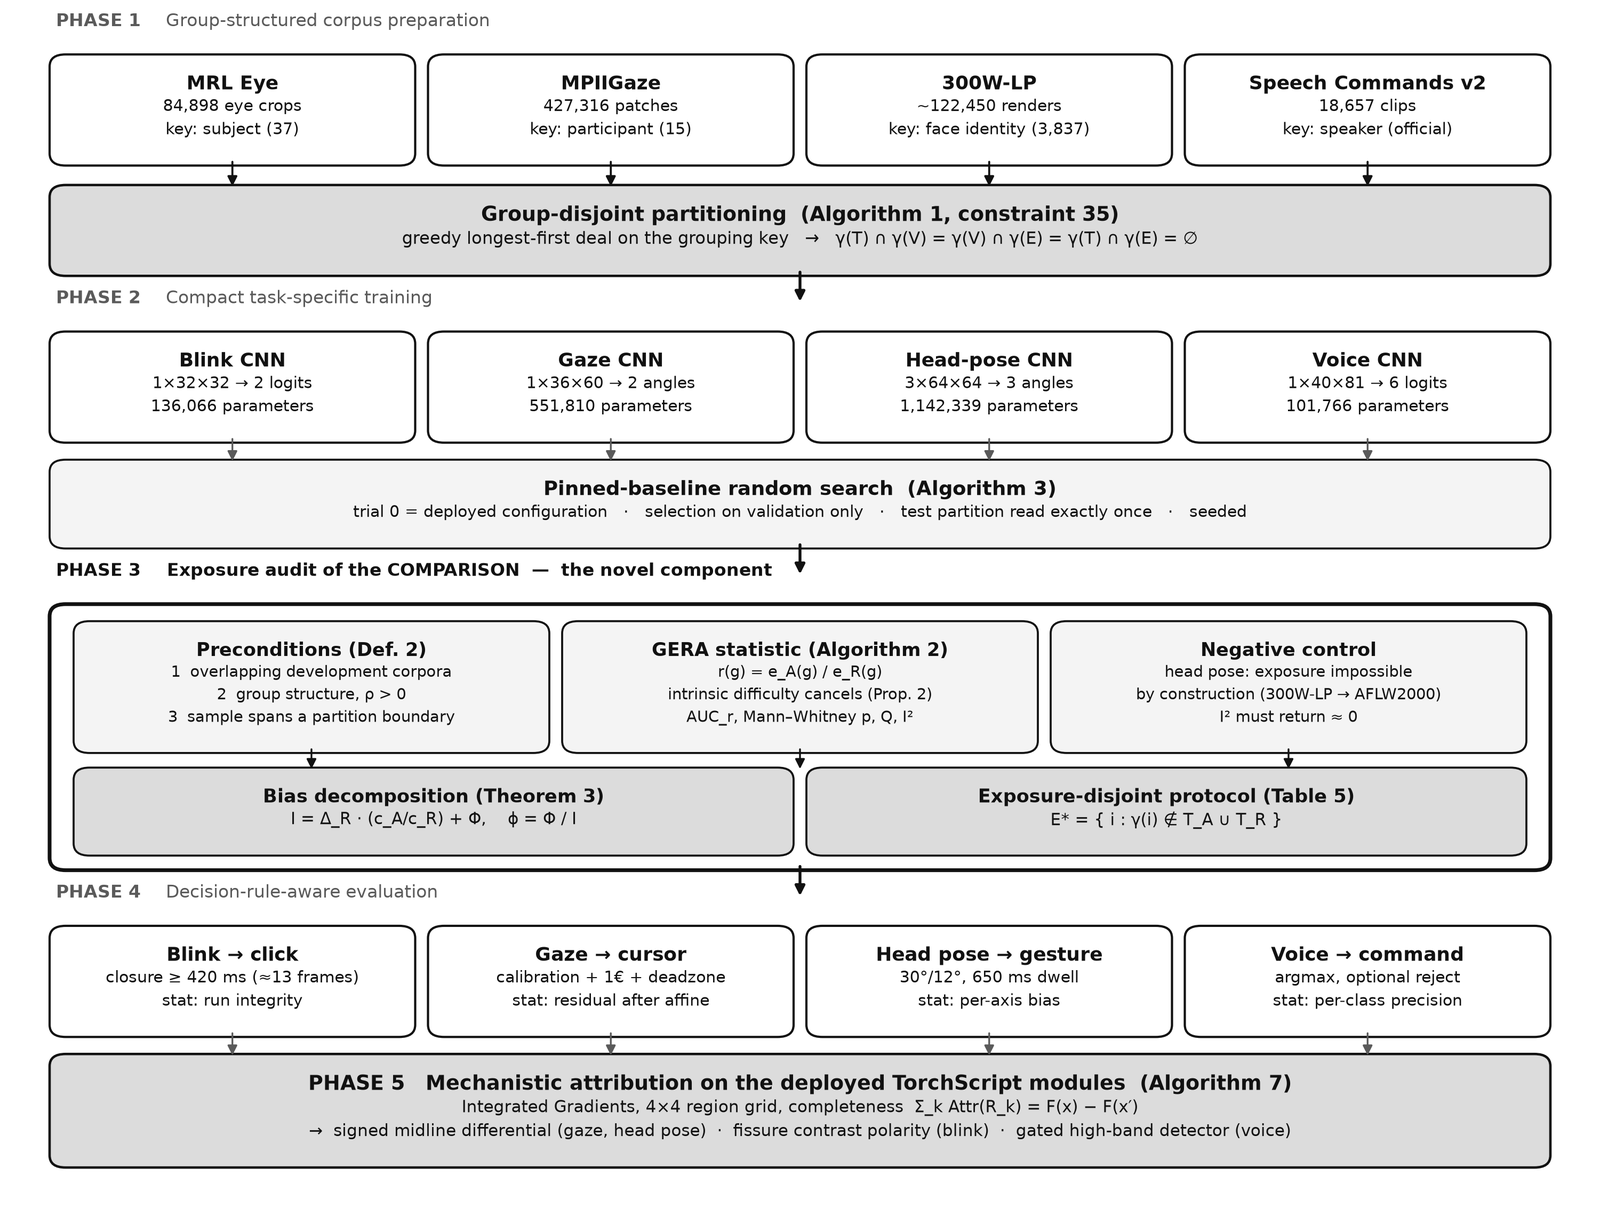
\includegraphics[width=\linewidth]{figures/protocol_P0_framework.png}
\caption{Overview of the MAPLE framework. Four group-structured corpora are partitioned by identity, feeding four compact task-specific networks trained under a pinned-baseline random search. Before any cross-model comparison is reported, the comparison itself is audited for asymmetric exposure by the GERA statistic against a reference model, with a negative control on a corpus where exposure is impossible by construction; only exposure-disjoint strata enter the reported contrast. Each network's error is then read through the deployed decision rule that consumes it, and Integrated-Gradients attribution on the shipped TorchScript modules identifies the operator each network computes.}
\label{fig:1}
\end{figure}

\FloatBarrier

\subsection{Problem formalisation}

\subsubsection{The interaction system as a composition}

Let the system observe, at discrete time \emph{t}, a camera frame \textbf{I}$_{t}$ $\in$ $\mathbb{R}^{(H \times W \times 3)}$ and an audio buffer \textbf{a}$_{t}$ $\in$ $\mathbb{R}^{L}$. A \emph{modality} m $\in$ $\mathcal{M}$ = \{blink, gaze, pose, voice\} is a pair ($f_{m}$, $\Delta_{m}$) consisting of a learned perception map $f_{m}$ and a deterministic decision rule $\Delta_{m}$. Writing $\mathcal{C}_{m}$ for the modality-specific crop or transform applied to the raw observation, the per-frame computation is

\begin{equation}
\label{eq:1}
\begin{aligned}
u_m, _{t} = f_m(\mathcal{C}_m(\mathbf{I}_{t}, \mathbf{a}_{t}) ; \vartheta _m), a_{m}, \\
_{t} = \Delta _m(u_m,_{t}, u_m,_{t-1}, \dots , u_m,_{t-}K ; \psi _m)
\end{aligned}
\end{equation}

where $\vartheta_{m}$ are the learned parameters, $\psi_{m}$ the decision-rule parameters (thresholds, dwell times, hysteresis bands, filter cut-offs), and $a_{m}$,$_{t}$ $\in$ $\mathcal{A}_{m}$ the emitted action, with $\mathcal{A}_{m}$ possibly containing a null action. The essential structural point, and the one that governs the entire evaluation design of Section 3.11, is that the user experiences the composite $\Delta_{m}$ $\circ$ $f_{m}$ and never $f_{m}$ alone. Consequently the loss under which $f_{m}$ is \emph{trained} and the statistic by which $f_{m}$ is \emph{usefully reported} need not coincide, and in three of the four modalities studied here they do not.

The complete system output at time \emph{t} is the arbitrated union

\begin{equation}
\label{eq:2}
\mathcal{S}(\mathbf{I}_{t}, \mathbf{a}_{t}) = \bigcup _{m \in \mathcal{M}} \Delta _m(f_m(\mathcal{C}_m(\mathbf{I}_{t}, \mathbf{a}_{t}))),
\end{equation}

subject to an arbitration relation that suppresses conflicting simultaneous actions (Section 3.9.5).

\subsubsection{The concurrency constraint}

The three vision modalities share a single face-landmark inference \CITE{mediapipe,facemesh} $\ell$(\textbf{I}$_{t}$), executed once per frame, whose output supplies the crops $\mathcal{C}_{\mathrm{blink}}$, $\mathcal{C}_{\mathrm{gaze}}$ and $\mathcal{C}_{\mathrm{pose}}$. Writing $\tau$($\cdot$) for wall-clock latency, real-time operation at frame rate F requires

\begin{equation}
\label{eq:3}
\tau (\ell ) + \Sigma _{m \in \mathcal{M}_{\mathrm{vis}}} [ \tau (\mathcal{C}_m) + \tau (f_m) + \tau (\Delta _m) ] + \tau (\text{stab}) \leq 1 / F
\end{equation}

with $\mathcal{M}_{\mathrm{vis}}$ = \{blink, gaze, pose\} and $\tau$(stab) the cursor stabilisation chain. At F = 30 Hz the budget is 33.3 ms. The voice modality runs on an independent audio thread and enters \EQREF{3} only through CPU contention, not through the frame-serial path. Inequality \EQREF{3} is the constraint that makes the \emph{sum} of model costs the binding quantity, and therefore the constraint under which an individual model's accuracy may rationally be traded.

\subsubsection{Risk, and why the empirical risk is the wrong target here}

For a modality with sample space $\mathcal{X}_{m}$ $\times$ $\mathcal{Y}_{m}$, distribution $\mathcal{D}_{m}$ and loss $\ell_{m}$, the population risk of a hypothesis f is

\begin{equation}
\label{eq:4}
R_m(f) = \mathbb{E}_{(x,y) \sim \mathcal{D}_m} [ \ell _m(f(x), y) ]
\end{equation}

estimated on a finite sample S = \{(x$_{i}$, y$_{i}$)\}$_{i=1}^{n}$ by

\begin{equation}
\label{eq:5}
\hat{R}_m(f ; S) = (1/n) \Sigma _{i=1}^{n} \ell _m(f(x_{i}), y_{i}).
\end{equation}

The estimator \EQREF{5} is unbiased for \EQREF{4} only when the sample is drawn i.i.d. from $\mathcal{D}_{m}$. In every corpus used here it is not: samples are organised into groups (a subject, a participant, a base face identity, a speaker) with strong within-group dependence, and the deployment distribution places the \emph{entire} group of a new user outside the training data. The relevant risk is therefore the group-conditional one,

\begin{equation}
\label{eq:6}
R_m^{\mathrm{grp}}(f) = \mathbb{E}_{g \sim \mathcal{G}} \mathbb{E}_{(x,y) \sim \mathcal{D}_m(\cdot | g)} [ \ell _m(f(x), y) ],
\end{equation}

where $\mathcal{G}$ is the population of groups. Equations \EQREF{5} and \EQREF{6} coincide only if the evaluation groups are disjoint from the training groups; Sections 3.4 and 3.5 are concerned with the two distinct ways in which that condition can fail.

\subsubsection{Notation}

\TABREF{3} fixes the notation used throughout. Modality subscripts are dropped wherever the context is unambiguous.

\begin{table}[pos=htbp]
\centering
\caption{Summary of mathematical notation.}
\label{tab:3}
\footnotesize
\begin{tabularx}{\textwidth}{XX}
\toprule
\textbf{Symbol} & \textbf{Description} \\
\midrule
$\mathcal{M}$, $\mathcal{M}_{\mathrm{vis}}$ & Set of modalities; the three vision modalities sharing one landmark inference \\
$f_{m}$($\cdot$ ; $\vartheta_{m}$) & Learned perception map of modality \emph{m} with parameters $\vartheta_{m}$ \\
$\Delta_{m}$($\cdot$ ; $\psi_{m}$) & Deployed decision rule consuming $f_{m}$, with parameters $\psi_{m}$ \\
$\mathcal{C}_{m}$ & Modality-specific crop / transform of the raw observation \\
$\mathcal{G}$, g & Population of groups; a single group (subject, participant, face identity, speaker) \\
$\gamma$(i) $\in$ $\mathcal{G}$ & Group label of sample \emph{i} \\
$\mathcal{T}_{A}$, $\mathcal{T}_{R}$ & Training-partition group sets of the audited and reference models \\
$\mathcal{V}$, $\mathcal{E}$ & Validation and evaluation index sets \\
A, R & Audited model and reference (control) model \\
$e_{A}$(i), $e_{R}$(i) & Per-sample error of the audited and reference model on sample \emph{i} \\
$\bar{e}_{A}$(g), $\bar{e}_{R}$(g) & Group-mean error of A and R on group \emph{g} \\
r(g) & Group error ratio $\bar{e}_{A}$(g) / $\bar{e}_{R}$(g) --- the GERA statistic \\
d(g) & Intrinsic difficulty of group \emph{g} \\
$c_{A}$, $c_{R}$ & Model-level capability constants \\
$\varphi$ & Familiarity discount enjoyed by a model on its own training groups \\
$\rho$ & Intraclass correlation of the loss within a group \\
n, $n_{g}$, G & Sample count; samples in group \emph{g}; number of groups \\
$n_{\mathrm{eff}}$ & Effective sample size after accounting for within-group dependence \\
$\pi$ & Per-group sampling quota vector of the evaluation sample \\
s & Fitted regression gain of predicted on true target (shrinkage gain) \\
$\theta$, $\hat{\theta }$ & True and predicted target (angle, in radians or degrees) \\
$\sigma^{2}$, $\sigma_{\varepsilon^{2}}$ & Target variance; irreducible representational noise variance \\
Q, I$^{2}$ & Cochran's heterogeneity statistic and the derived inconsistency index \\
$\alpha_{\mathrm{OE}}$, $\beta$, $f_{c}$ & One-euro filter smoothing factor, speed coefficient, cut-off \\
\textbf{w}, \textbf{P}, $\lambda_{f}$ & Calibration weights, RLS inverse-covariance, forgetting factor \\
$T_{\mathrm{hold}}$, $T_{\mathrm{dwell}}$, $T_{\mathrm{cd}}$ & Blink hold threshold, gesture dwell time, cooldown \\
$\theta_{\mathrm{on}}$, $\theta_{\mathrm{off}}$ & Gesture trigger and release thresholds (hysteresis band) \\
$\mathcal{A}_{m}$ & Action alphabet of modality \emph{m} \\
\bottomrule
\end{tabularx}
\end{table}

\FloatBarrier

\subsection{Corpora, grouping keys and evaluation sets}

Four public corpora supply the four modalities. Each is assigned an explicit grouping key, and that assignment is the precondition for everything that follows: a corpus with group structure and within-group dependence is exactly a corpus in which both leakage faults of Section 3.4 and Section 3.5 can occur.

\begin{table}[pos=htbp]
\centering
\caption{Corpora, grouping keys and evaluation sets.}
\label{tab:4}
\footnotesize
\begin{tabularx}{\textwidth}{XXXXXX}
\toprule
\textbf{Modality} & \textbf{Training corpus} & \textbf{Evaluation set} & \textbf{N} & \textbf{Grouping key} & \textbf{Groups} \\
\midrule
Blink & MRL Eye Dataset (84,898 greyscale/IR eye crops) & Held-out subjects & 12,927 & Subject identity & 37 \\
Gaze & MPIIGaze, normalised patches (427,316) & Held-out participants & 64,172 & Participant & 15 \\
Head pose & 300W-LP (\textasciitilde{}122,450 synthesised renders) & AFLW2000, untouched & 1,969 & Base face identity & 3,837 \\
Voice & Speech Commands v2 (18,657 clips, 6 keywords) & Official test list & 2,468 & Speaker & official \\
\bottomrule
\end{tabularx}
\end{table}

\subsubsection{Within-group dependence and effective sample size}

Let $\ell_{i}$ = $\ell$(f(x$_{i}$), y$_{i}$) denote the per-sample loss and let $\gamma$(i) be the group label. Model the loss by a one-way random-effects decomposition

\begin{equation}
\label{eq:7}
\begin{aligned}
\ell _{i} = \mu + b_{\gamma (i)} + \varepsilon _{i}, b_g \sim (0, \sigma _b^{2}), \\
\varepsilon _{i} \sim (0, \sigma _w^{2}),
\end{aligned}
\end{equation}

with b and $\varepsilon$ independent. The intraclass correlation of the loss \CITE{kish} is then

\begin{equation}
\label{eq:8}
\rho = \sigma _b^{2} / (\sigma _b^{2} + \sigma _w^{2}),
\end{equation}

and for a sample containing G groups of equal size $\bar{n}$ = n/G the variance of the sample mean loss is inflated relative to the i.i.d. case by the design effect

\begin{equation}
\label{eq:9}
\begin{aligned}
\mathrm{Var}(\bar{\ell }) = (\sigma _b^{2} + \sigma _w^{2})/n \cdot [ 1 + (\bar{n} - 1) \rho ], \\
\mathrm{DEFF} = 1 + (\bar{n} - 1) \rho ,
\end{aligned}
\end{equation}

so that the effective sample size is

\begin{equation}
\label{eq:10}
n_{\mathrm{eff}} = n / [ 1 + (\bar{n} - 1) \rho ].
\end{equation}

Equation \EQREF{10} is the quantitative statement of why a corpus with thousands of frames per participant does not supply thousands of independent observations, and why the number of \emph{groups} rather than the number of \emph{rows} is the sample size that governs a cross-person claim. For the gaze evaluation of Section 5.2, n = 64,172 rows drawn from G = 2 held-out participants gives $n_{\mathrm{eff}}$ $\to$ 2/$\bar{\rho }$ as $\bar{n}$ grows, which is why Section 6 records the held-out participant count as the principal limitation of the study notwithstanding the large row count.

\subsubsection{The leakage probability under random row splitting}

Consider partitioning n rows uniformly at random into a training fraction p and a test fraction 1 -- p, ignoring group structure. For a test row i belonging to a group of size $n_{g}$, the probability that at least one row of the same group falls in the training partition is

\begin{equation}
\label{eq:11}
\mathbb{P}[ \text{leak}\;(i) ] = 1 - (1 - p)^{n_g - 1} ,
\end{equation}

which for the corpora of \TABREF{4} is numerically indistinguishable from unity: with p = 0.7 and $n_{g}$ = 2,300 (MRL), 1 -- $0.3^{2299}$ < $10^{-1200}$. Under random row splitting essentially \emph{every} test row has a near-duplicate exemplar of the same individual available in training, and the expected fraction of the test set that is contaminated in this sense is

\begin{equation}
\label{eq:12}
\mathbb{E}[ \text{contaminated fraction} ] = (1/n) \Sigma _{i=1}^{n} [ 1 - (1 - p)^{n_{\gamma (i)} - 1} ] \approx 1.
\end{equation}

The measured consequence is reported in Section 5.1: replacing random row splitting by group-disjoint splitting costs 5.81 pp of blink accuracy and 4.11$^{\circ}$ of gaze angular error, while leaving head pose and voice --- whose evaluation sets are group-disjoint by construction --- unchanged to within the seed-to-seed noise floor.

\FloatBarrier

\subsection{Preprocessing and input representations}

Each modality applies a deterministic transform $\mathcal{C}_{m}$ from raw observation to network input. All transforms are implemented identically in the training scripts and in the deployed providers, with the single documented exception noted in Section 5.2.1.

\subsubsection{Eye-region extraction and photometric normalisation (blink)}

Given the landmark set $\mathcal{L}$(\textbf{I}) returned by the shared face-landmark inference, the eye region is the axis-aligned bounding box of the palpebral landmark subset $\mathcal{L}_{\mathrm{eye}}$, expanded by a margin $\kappa$ and resampled to the canonical size 32 $\times$ 32:

\begin{equation}
\label{eq:13}
\mathbf{b} = [ \mathrm{min}_x \mathcal{L}_{\mathrm{eye}} - \kappa w, \mathrm{min}_y \mathcal{L}_{\mathrm{eye}} - \kappa h, \mathrm{max}_x \mathcal{L}_{\mathrm{eye}} + \kappa w, \mathrm{max}_y \mathcal{L}_{\mathrm{eye}} + \kappa h ],
\end{equation}

\begin{equation}
\label{eq:14}
x_{\mathrm{blink}} = \mathrm{Resize}_{32\times 32} ( \mathrm{Gray} ( \mathbf{I} [ \mathbf{b} ] ) ) / 255 \in [0,1]^{32\times 32}.
\end{equation}

Photometric normalisation applies per-crop standardisation, which removes the additive and multiplicative illumination terms that dominate variation across sessions and devices:

\begin{equation}
\label{eq:15}
\begin{aligned}
\tilde{x} = ( x - \mu _x ) / ( \sigma _x + \epsilon ), \\
\mu _x = (1/|x|) \Sigma _{u} x_u, \\
\sigma _x^{2} = (1/|x|) \Sigma _{u} (x_u - \mu _x)^{2},
\end{aligned}
\end{equation}

with $\epsilon$ = 10$^{-6}$ guarding degenerate crops. Section 5.5 shows via attribution that the network subsequently learns a \emph{contrast-polarity} code over the central fissure region, which is precisely the representation for which \EQREF{15} is the correct normalisation, since a polarity code is invariant to the affine photometric family that \EQREF{15} quotients out.

\subsubsection{Gaze patch normalisation and angular parameterisation}

MPIIGaze supplies eye patches already normalised by the standard procedure, which applies a virtual camera rotation \textbf{R}\_n and scaling \textbf{S}\_n such that the eye centre lies on the optical axis at fixed distance and the eye's horizontal axis is image-aligned:

\begin{equation}
\label{eq:16}
\begin{aligned}
\mathbf{M} = \mathbf{S}_n \mathbf{R}_n, \\
x_{\mathrm{gaze}} = \mathrm{Warp}_{\mathbf{M}} ( \mathrm{Gray} ( \mathbf{I} ) ) \in \mathbb{R}^{36\times 60}.
\end{aligned}
\end{equation}

The corpus annotates a 3-D gaze unit vector \textbf{g} = ($g_{x}$, $g_{y}$, $g_{z}$)$^{\mathsf{T}}$ in the normalised camera frame, converted to the pitch--yaw parameterisation the network regresses:

\begin{equation}
\label{eq:17}
\hat{\mathbf{g}} = \mathbf{g} / ( \|\mathbf{g}\|_{2} + \epsilon ),
\end{equation}

\begin{equation}
\label{eq:18}
\begin{aligned}
\theta _{\mathrm{pitch}} = \arcsin( - \hat{g}_y ), \\
\theta _{\mathrm{yaw}} = \arctan2( - \hat{g}_x , - \hat{g}_z ).
\end{aligned}
\end{equation}

The inverse map, used to recover a direction from a prediction for angular-error computation, is

\begin{equation}
\label{eq:19}
\mathbf{g}(\theta _{\mathrm{pitch}}, \theta _{\mathrm{yaw}}) = ( - \cos \theta _{\mathrm{pitch}} \sin \theta _{\mathrm{yaw}} , - \sin \theta _{\mathrm{pitch}} , - \cos \theta _{\mathrm{pitch}} \cos \theta _{\mathrm{yaw}} )^{\mathsf{T}}.
\end{equation}

Angular error between a prediction and ground truth is computed on the sphere rather than in the parameter plane, since the parameter plane is not isometric:

\begin{equation}
\label{eq:20}
e_{\mathrm{ang}} = \arccos ( \mathrm{clip}_{[-1,1]} ( \mathbf{g}(\hat{\theta }) \cdot \mathbf{g}(\theta ) ) ) \cdot 180/\pi [\text{degrees}].
\end{equation}

Equation \EQREF{20} is the statistic reported throughout as ``angular error''; the separately reported ``MAE'' is the mean absolute error in the (pitch, yaw) parameter plane,

\begin{equation}
\label{eq:21}
\mathrm{MAE} = (1/2n) \Sigma _{i=1}^{n} ( |\hat{\theta }_{\mathrm{pitch}},i - \theta _{\mathrm{pitch}},i| + |\hat{\theta }_{\mathrm{yaw}},i - \theta _{\mathrm{yaw}},i| ) \cdot 180/\pi ,
\end{equation}

and the two are reported together because they respond differently to the shrinkage mechanism of Section 5.2.2: \EQREF{20} is a chordal quantity that grows with eccentricity, \EQREF{21} a per-axis quantity that does not.

\subsubsection{Face crop and head-pose parameterisation}

The head-pose network consumes a square RGB crop derived from the 68-point landmark set, expanded to include the full facial envelope:

\begin{equation}
\label{eq:22}
\begin{aligned}
c = ( (\mathrm{min}_x + \mathrm{max}_x)/2 , (\mathrm{min}_y + \mathrm{max}_y)/2 ), \\
\ell _{\mathrm{side}} = (1 + \kappa _f) \cdot \mathrm{max}( \mathrm{max}_x - \mathrm{min}_x , \mathrm{max}_y - \mathrm{min}_y ),
\end{aligned}
\end{equation}

\begin{equation}
\label{eq:23}
x_{\mathrm{pose}} = \mathrm{Resize}_{64\times 64} ( \mathbf{I} [ c \pm \ell _{\mathrm{side}}/2 ] ) \in \mathbb{R}^{3\times 64\times 64}.
\end{equation}

Ground-truth pose is supplied as intrinsic Euler angles (pitch, yaw, roll) = ($\theta_{p}$, $\theta_{y}$, $\theta_{r}$), which define the rotation

\begin{equation}
\label{eq:24}
\mathbf{R} = \mathbf{R}_z(\theta _r) \mathbf{R}_y(\theta _y) \mathbf{R}_x(\theta _p),
\end{equation}

with the usual elementary rotations

\begin{equation}
\label{eq:25}
\begin{aligned}
\mathbf{R}_x(a) = \begin{bmatrix} 1 & 0 & 0 \\ 0 & \cos a & -\sin a \\ 0 & \sin a & \cos a \end{bmatrix}, \\
\mathbf{R}_y(a) = \begin{bmatrix} \cos a & 0 & \sin a \\ 0 & 1 & 0 \\ -\sin a & 0 & \cos a \end{bmatrix}, \\
\mathbf{R}_z(a) = \begin{bmatrix} \cos a & -\sin a & 0 \\ \sin a & \cos a & 0 \\ 0 & 0 & 1 \end{bmatrix}.
\end{aligned}
\end{equation}

The network regresses ($\theta_{y}$, $\theta_{p}$, $\theta_{r}$) in degrees directly. Samples with max(|$\theta_{y}$|, |$\theta_{p}$|, |$\theta_{r}$|) > 99$^{\circ}$ are excluded, following the standard protocol, because beyond that range the projected facial evidence is largely self-occluded and the annotation itself becomes unreliable; Section 5.3 shows that error nevertheless grows sharply well inside this bound and identifies the occlusion mechanism responsible.

Horizontal flip augmentation is \emph{not} label-preserving for this task, and applying it naively is a silent correctness fault. The correct paired transform is

\begin{equation}
\label{eq:26}
( x , (\theta _y, \theta _p, \theta _r) ) \mapsto ( \text{flip}\;_h(x) , (-\theta _y, \theta _p, -\theta _r) ),
\end{equation}

and Section 5.3 reports the diagnostic that confirms it was applied correctly: the per-band error distributions broaden and shift together rather than becoming bimodal, whereas sign confusion from an uncorrected flip would produce bimodality.

\subsubsection{Log-mel acoustic front end}

Audio is resampled to $F_{s}$ = 16 kHz and reduced to a fixed one-second window by right-padding or truncation:

\begin{equation}
\label{eq:27}
a'[n] = a[n] \cdot \mathbf{1}[ n < \mathrm{min}(L, F_s) ] , n = 0, \dots , F_s - 1.
\end{equation}

The short-time Fourier transform \CITE{welch} uses $N_{\mathrm{fft}}$ = 400 (25 ms) with hop H = 200 (12.5 ms), giving T = 81 frames:

\begin{equation}
\label{eq:28}
X[k, \tau ] = \Sigma _{n=0}^{N_{\mathrm{fft}} - 1} a'[ \tau H + n ] \cdot w[n] \cdot \mathrm{exp}( -j 2\pi k n / N_{\mathrm{fft}} ),
\end{equation}

with w a Hann window. The power spectrum is projected onto B = 40 mel-spaced triangular filters,

\begin{equation}
\label{eq:29}
\mathrm{mel}(f) = 2595 \cdot \mathrm{log}_{10}( 1 + f/700 ),
\end{equation}

\begin{equation}
\label{eq:30}
\begin{aligned}
H_b[k] = \mathrm{triangular} \;\text{filter b}, \;\text{centred at} \\ 
\mathrm{mel}^{-1}( \mathrm{mel}(f_{\mathrm{low}}) + b \cdot ( \mathrm{mel}(f_{\mathrm{high}}) - \mathrm{mel}(f_{\mathrm{low}}) ) / (B+1) ),
\end{aligned}
\end{equation}

\begin{equation}
\label{eq:31}
M[b, \tau ] = \Sigma _{k} H_b[k] \cdot | X[k, \tau ] |^{2} ,
\end{equation}

and compressed logarithmically to give the network input

\begin{equation}
\label{eq:32}
\begin{aligned}
x_{\mathrm{voice}}[b, \tau ] = \mathrm{log}( M[b, \tau ] + \epsilon ) , \\
\epsilon = 10^{-6} , x_{\mathrm{voice}} \in \mathbb{R}^{1 \times 40 \times 81}.
\end{aligned}
\end{equation}

The logarithm in \EQREF{32} is what makes the representation approximately invariant to recording gain, since a multiplicative gain becomes an additive offset that the first convolution's bias and the subsequent batch normalisation absorb. Section 5.4 shows via attribution that the network learns an implicit voice-activity gate over the time axis of \EQREF{32} --- concentrating attribution on central time slots and discarding the silence padding --- which is the property that permits transfer to a live microphone stream whose padding statistics differ from the corpus.

\subsubsection{The augmentation operator family}

Augmentation is modelled as a distribution over label-preserving (or label-covariantly-transformed) operators. Writing $\mathcal{A}$ = \{$T_{\omega}$ : $\omega$ $\sim$ $p_{\omega}$\} for the family, training minimises the augmented risk

\begin{equation}
\label{eq:33}
\hat{R}^{\mathrm{aug}}(f ; S) = (1/n) \Sigma _{i=1}^{n} \mathbb{E}_{\omega \sim p_{\omega} } [ \ell ( f(T_{\omega} (x_{i})), \mathcal{T}_{\omega} (y_{i}) ) ] ,
\end{equation}

where $\mathcal{T}_{\omega}$ is the induced label transform --- the identity for blink and voice, the sign flip of \EQREF{26} for head pose, and yaw negation for gaze. The operator family used for the gaze domain-shift correction of Section 5.2.1 is constructed to model the \emph{specific} deterministic shift between normalised training patches and landmark-cropped inference regions, and is therefore analytic rather than generic:

\begin{equation}
\label{eq:34}
\begin{aligned}
T_{\omega} = \mathrm{Rot}(\delta ) \circ \mathrm{Jitter}(\alpha , \beta ) \circ \mathrm{Blur}(\sigma _b) , \\
\delta \sim \mathcal{U}(-8^{\circ}, +8^{\circ}), \alpha \sim \mathcal{U}(0.8, 1.2), \\
\beta \sim \mathcal{U}(-0.2, 0.2), \\
\sigma _b \sim \mathcal{U}(0, \sigma _{\mathrm{max}}),
\end{aligned}
\end{equation}

with Jitter($\alpha$, $\beta$) applying x $\mapsto$ clip($\alpha$ x + $\beta$), Blur($\sigma_{b}$) a Gaussian kernel modelling sensor resolution loss, and Rot($\delta$) an in-plane rotation modelling residual head roll. Because every member of \EQREF{34} is label-preserving up to the flip correction, any gain it produces cannot be additional supervision; it is an enlargement of the effective input manifold at zero parameter and zero data cost. Section 5.2.1 measures a 9.5 \% reduction in \emph{both} a robust and a non-robust error statistic, which is the signature of removing a distributional mismatch rather than repairing isolated failures.

\FloatBarrier

\subsection{First-order leakage: group-disjoint partitioning}

\subsubsection{The partition constraint}

Let the index set be [n] = \{1, $\dots$, n\} with group labels $\gamma$ : [n] $\to$ $\mathcal{G}$. A three-way partition ([n] = $\mathcal{T}$ $\uplus$ $\mathcal{V}$ $\uplus$ $\mathcal{E}$) is \emph{group-disjoint} if

\begin{equation}
\label{eq:35}
\begin{aligned}
\gamma (\mathcal{T}) \cap \gamma (\mathcal{V}) = \emptyset , \\
\gamma (\mathcal{V}) \cap \gamma (\mathcal{E}) = \emptyset , \\
\gamma (\mathcal{T}) \cap \gamma (\mathcal{E}) = \emptyset ,
\end{aligned}
\end{equation}

that is, no group contributes rows to more than one part. Under \EQREF{35} the evaluation estimator \EQREF{5} is an unbiased estimate of the group-conditional risk \EQREF{6} restricted to the evaluation groups, whereas under random row splitting it estimates a mixture that Section 3.5.2 makes explicit.

Because group sizes are highly unequal --- MRL subjects span roughly 700 to 10,000 frames --- a partition that is group-disjoint need not be close to the target row fractions. We therefore deal groups greedily in decreasing size order into whichever part is furthest below its row target, which is the classical longest-processing-time-first heuristic for multiway number partitioning \CITE{graham}:

\begin{equation}
\label{eq:36}
\begin{aligned}
\text{part}\;(g) = \mathrm{arg\,\mathrm{max}}_{j \in {1,2,3}} ( n \cdot \varphi _j - c_j ), \\
c_j \leftarrow c_j + n_g ,
\end{aligned}
\end{equation}

with $\varphi$ = (0.70, 0.15, 0.15) the target fractions and $c_{j}$ the running row count of part \emph{j}. The heuristic admits the standard bound: for group sizes $n_{(1)}$ $\geq$ $n_{(2)}$ $\geq$ $\dots$ the maximum deviation of any part from its target satisfies

\begin{equation}
\label{eq:37}
| c_j - n \varphi _j | \leq \mathrm{max}_g n_g ,
\end{equation}

which is tight in the worst case but far from tight in practice; the realised deviations for all four corpora are below 5 \% of n. \ALGREF{1} states the procedure.

\begin{algorithm}[htbp]
\caption{Group-disjoint partitioning (greedy longest-first deal)}
\label{alg:1}
\hrule\vspace{3pt}
{\ttfamily\scriptsize\raggedright
Require: group labels $\gamma$(1..n); target fractions $\varphi$ = ($\varphi_{1}$, $\varphi_{2}$, $\varphi_{3}$) with $\Sigma \varphi_{j}$ = 1; seed $\sigma$ \\
Ensure: index sets $\mathcal{T}$, $\mathcal{V}$, $\mathcal{E}$ satisfying the disjointness constraint (35) \\
~1: $\mathcal{U}$ $\leftarrow$ unique($\gamma$);~~rng $\leftarrow$ RandomState($\sigma$);~~shuffle($\mathcal{U}$, rng) \\
~2: for all g $\in$ $\mathcal{U}$ do $n_{g}$ $\leftarrow$ |\{ i : $\gamma$(i) = g \}| end for \\
~3: targets $\leftarrow$ (n$\cdot\varphi_{1}$, n$\cdot\varphi_{2}$, n$\cdot\varphi_{3}$);~~counts $\leftarrow$ (0, 0, 0);~~buckets $\leftarrow$ ($\emptyset$, $\emptyset$, $\emptyset$) \\
~4: for all g $\in$ sort($\mathcal{U}$, key = --$n_{g}$) do~~~~~~~~~~~~~~~~~~~~$\triangleright$ largest group first \\
~5:~~~~~j $\leftarrow$ arg $max_{j \in \{1,2,3}$\} ( targets[j] -- counts[j] )~~$\triangleright$ furthest below target \\
~6:~~~~~buckets[j] $\leftarrow$ buckets[j] $\cup$ \{g\};~~counts[j] $\leftarrow$ counts[j] + $n_{g}$ \\
~7: end for \\
~8: $\mathcal{T}$ $\leftarrow$ \{ i : $\gamma$(i) $\in$ buckets[1] \};~~$\mathcal{V}$ $\leftarrow$ \{ i : $\gamma$(i) $\in$ buckets[2] \};~~$\mathcal{E}$ $\leftarrow$ \{ i : $\gamma$(i) $\in$ buckets[3] \} \\
~9: assert $\gamma$($\mathcal{T}$) $\cap$ $\gamma$($\mathcal{V}$) = $\gamma$($\mathcal{V}$) $\cap$ $\gamma$($\mathcal{E}$) = $\gamma$($\mathcal{T}$) $\cap$ $\gamma$($\mathcal{E}$) = $\emptyset$ \\
10: assert $\mathcal{T}$ $\uplus$ $\mathcal{V}$ $\uplus$ $\mathcal{E}$ = [n] \\
11: return $\mathcal{T}$, $\mathcal{V}$, $\mathcal{E}$
\par}
\vspace{3pt}\hrule
\end{algorithm}

The grouping keys are, per corpus: the subject identifier encoded in the MRL filename; the participant identifier p00--p14 for MPIIGaze; the base face identity for 300W-LP, recovered by stripping the synthesised view index and flip tag from the filename so that all renders of one face share a key; and, for Speech Commands, the official validation and testing lists, which are already speaker-aware and therefore require no custom grouping.

\subsubsection{What the correction is worth, and the internal control}

Three quantities are reported per modality throughout this work: the \emph{published} score obtained under the faulty random-row protocol; the \emph{fair baseline}, retraining the original hyperparameters under the corrected protocol; and the \emph{tuned} score under that same corrected protocol. Separating the three is what prevents the protocol effect and the optimisation effect from being conflated, a conflation that would otherwise make it impossible to attribute any reported improvement.

Two of the four modalities have evaluation sets that are group-disjoint by construction and receive no partition change at all --- head pose is evaluated on AFLW2000, disjoint from 300W-LP by design, and voice uses the official speaker-disjoint split --- so either could in principle serve as an \emph{internal negative control} on the correction itself. If group-disjoint partitioning merely depressed scores indiscriminately, an unchanged partition would nonetheless fall along with the changed ones. Section 5.1.1 reports that head pose moves by less than the seed-to-seed noise floor and therefore does serve as that control, which is what licenses attributing the blink and gaze corrections to leakage rather than to a stricter protocol in general; a single-modality study could not supply it. It also reports that the voice figure moves by 7.24 pp despite an unchanged partition, for reasons this study does not establish, and voice is therefore \textbf{not} relied on as a second control. The control rests on head pose alone, and the reader should weigh it accordingly.

\FloatBarrier

\subsection{Second-order leakage: asymmetric exposure between compared models}

After the correction of Section 3.4 every pipeline in this work is group-disjoint and every model's individually reported score is sound. The \emph{comparison} between them is nevertheless still contaminated, because the fault does not live in either pipeline. It lives in the join.

\subsubsection{Formalisation}

\textbf{Definition 1 (Exposure set).} For a model M evaluated on a sample drawn from group population $\mathcal{G}$, the \emph{exposure set} $\mathcal{T}_{M}$ $\subseteq$ $\mathcal{G}$ is the set of groups whose data entered M's training partition. A group g is \emph{exposed} to M if g $\in$ $\mathcal{T}_{M}$.

\textbf{Definition 2 (Asymmetric exposure).} A comparison between models A and R on an evaluation sample $\mathcal{E}$ with group labels $\gamma$($\mathcal{E}$) $\subseteq$ $\mathcal{G}$ is \emph{asymmetrically exposed} when the following three conditions hold simultaneously:

\begin{enumerate}
\item \textbf{(Overlapping development corpora)} A and R were developed on corpora with non-empty intersection at the group level: $\mathcal{T}_{A}$ $\cap$ $\mathcal{T}_{R}$ $\neq$ $\emptyset$ or both derive from a common corpus;
\item \textbf{(Group structure with within-group dependence)} the corpus carries a grouping key with intraclass loss correlation $\rho$ > 0 in the sense of \EQREF{8};
\item \textbf{(Boundary-spanning evaluation sample)} the evaluation sample is drawn from groups on both sides of at least one model's partition boundary: $\gamma$($\mathcal{E}$) $\cap$ $\mathcal{T}_{A}$ $\neq$ $\emptyset$ \textbf{and} $\gamma$($\mathcal{E}$) \textbackslash\{\} $\mathcal{T}_{A}$ $\neq$ $\emptyset$ (or the same with $\mathcal{T}_{R}$).
\end{enumerate}

Condition 3 is the operative one and the one that per-pipeline auditing cannot see: it is a statement about the relation between the evaluation sample and \emph{the other model's} partition, and neither pipeline's own audit has any representation of that partition.

\textbf{Theorem 1 (Mixture representation and quota sensitivity).} Let A be a model with exposure set $\mathcal{T}_{A}$, and let the evaluation sample allocate a fraction $\pi_{g}$ of its mass to group g, with $\Sigma_{g}$ $\pi_{g}$ = 1. Define the exposed mass

\begin{equation}
\label{eq:38}
\Pi = \Sigma _{g \in \gamma (\mathcal{E}) \cap \mathcal{T}_A} \pi _g \in (0, 1).
\end{equation}

Then the reported aggregate error of A decomposes as the convex combination

\begin{equation}
\label{eq:39}
\bar{E}_A(\pi ) = \Pi \cdot \bar{E}_A^{\mathrm{in}} + (1 - \Pi ) \cdot \bar{E}_A^{\mathrm{out}},
\end{equation}

where $\bar{E}_{A}^{\mathrm{in}}$ and $\bar{E}_{A}^{\mathrm{out}}$ are the exposed- and unexposed-stratum means, each formed by averaging $\bar{e}_{A}$(g) over the groups of its own stratum under the weights $\pi_{g}$ renormalised to sum to one. Consequently

\begin{equation}
\label{eq:40}
\partial \bar{E}_A / \partial \Pi = \bar{E}_A^{\mathrm{in}} - \bar{E}_A^{\mathrm{out}} ,
\end{equation}

and whenever $\bar{E}_{A}^{\mathrm{in}}$ $\neq$ $\bar{E}_{A}^{\mathrm{out}}$ the reported error is a strictly monotone function of the sampling quota $\Pi$ alone. In particular, a change to the per-group sampling quota changes the reported accuracy without changing any model, any datum, or any metric definition.

\emph{Proof.} Write the sample mean error as a group-weighted mean, $\bar{e}_{A}$ = $\Sigma_{g}$ $\pi_{g}$ $\bar{e}_{A}$(g). Split the index set of groups by membership in $\mathcal{T}_{A}$ and factor the exposed mass $\Pi$ out of the first sum and (1 -- $\Pi$) out of the second; this yields \EQREF{39} directly, since the renormalised weights within each stratum sum to one by construction. Differentiating \EQREF{39} in $\Pi$, holding the two conditional means fixed, gives \EQREF{40}. Monotonicity is immediate from the sign of \EQREF{40}. $\blacksquare$

Theorem 1 states precisely what is objectionable. Under Definition 2 the aggregate is a mixture of a \emph{memorisation} regime and a \emph{generalisation} regime, with the mixing weight fixed by a sampling decision rather than by the research question. Two honest evaluators applying the same metric to the same models on the same corpus can report different numbers, and neither is making an error in the ordinary sense.

\textbf{Corollary 1 (Bias of the reported contrast).} Let the quantity of interest be the true cross-group contrast $\Delta$* = $\bar{E}_{A}^{\mathrm{out}}$ -- $\bar{E}_{R}^{\mathrm{out}}$, and let the reported contrast be $\hat{\Delta }$ = $\bar{E}_{A}$($\pi$) -- $\bar{E}_{R}$($\pi$). If R has no differential familiarity across $\gamma$($\mathcal{E}$) --- that is, $\bar{E}_{R}^{\mathrm{in}}$ = $\bar{E}_{R}^{\mathrm{out}}$ --- then

\begin{equation}
\label{eq:41}
\hat{\Delta } - \Delta * = \Pi \cdot ( \bar{E}_A^{\mathrm{in}} - \bar{E}_A^{\mathrm{out}} ) \leq 0,
\end{equation}

so the reported contrast understates A's true disadvantage by exactly the exposed mass times the within-model familiarity gap. The bias is signed, and it always favours the exposed model.

\emph{Proof.} Substitute \EQREF{39} for both models into $\hat{\Delta }$, apply $\bar{E}_{R}^{\mathrm{in}}$ = $\bar{E}_{R}^{\mathrm{out}}$ so that $\bar{E}_{R}$($\pi$) = $\bar{E}_{R}^{\mathrm{out}}$, and subtract $\Delta$*. The sign follows from $\bar{E}_{A}^{\mathrm{in}}$ $\leq$ $\bar{E}_{A}^{\mathrm{out}}$, which holds whenever training exposure does not increase error. $\blacksquare$

Corollary 1 is the reason Section 5 reports every comparison on the exposure-disjoint stratum only, and the reason a baseline trained on the whole corpus must be reported as a \emph{lower bound} on its own cross-person error rather than as a point estimate (protocol step 5, Section 3.5.6).

\subsubsection{The GERA statistic}

An auditor examining a published comparison rarely knows how either model was partitioned. The detector proposed here requires only what such an audit does have: the two prediction streams over a shared evaluation set, and a group label per sample.

\textbf{Definition 3 (Group error ratio).} For each group g $\in$ $\gamma$($\mathcal{E}$), let

\begin{equation}
\label{eq:42}
\begin{aligned}
\bar{e}_A(g) = (1/n_g) \Sigma _{i : \gamma (i) = g} e_A(i), \\
\bar{e}_R(g) = (1/n_g) \Sigma _{i : \gamma (i) = g} e_R(i),
\end{aligned}
\end{equation}

and define the \textbf{group error ratio}

\begin{equation}
\label{eq:43}
r(g) = \bar{e}_A(g) / \bar{e}_R(g).
\end{equation}

The role of R is to calibrate intrinsic group difficulty. Some groups are simply harder than others --- a fact A's own errors cannot separate from familiarity --- and a reference model with no \emph{differential} familiarity across those groups supplies exactly that missing control, because its across-group variation is intrinsic difficulty alone.

\textbf{Proposition 2 (Exact cancellation of intrinsic difficulty).} Suppose per-group errors follow the multiplicative difficulty model

\begin{equation}
\label{eq:44}
\begin{aligned}
\bar{e}_M(g) = d(g) \cdot c_M \cdot ( 1 - \varphi _M \cdot \mathbf{1}[ g \in \mathcal{T}_M ] ) , \\
M \in {A, R},
\end{aligned}
\end{equation}

with d(g) > 0 the intrinsic difficulty of group g, $c_{M}$ > 0 a model-level capability constant, and $\varphi_{M}$ $\in$ [0,1) the familiarity discount M enjoys on its own training groups. Then

\begin{equation}
\label{eq:45}
r(g) = ( c_A / c_R ) \cdot ( 1 - \varphi _A \mathbf{1}[ g \in \mathcal{T}_A ] ) / ( 1 - \varphi _R \mathbf{1}[ g \in \mathcal{T}_R ] ),
\end{equation}

which is free of d(g). If in addition R has no differential familiarity across $\gamma$($\mathcal{E}$) --- either $\mathcal{T}_{R}$ $\supseteq$ $\gamma$($\mathcal{E}$) or $\mathcal{T}_{R}$ $\cap$ $\gamma$($\mathcal{E}$) = $\emptyset$, so the indicator is constant --- then

\begin{equation}
\label{eq:46}
\begin{aligned}
r(g) = \kappa \cdot ( 1 - \varphi _A \mathbf{1}[ g \in \mathcal{T}_A ] ), \\
\kappa = ( c_A / c_R ) / ( 1 - \varphi _R \mathbf{1}[\gamma (\mathcal{E}) \subseteq \mathcal{T}_R] ) ,
\end{aligned}
\end{equation}

so r(g) takes exactly two values, $\kappa$(1 -- $\varphi_{A}$) on exposed groups and $\kappa$ on unexposed groups, and the ratio of the two group means identifies the familiarity discount:

\begin{equation}
\label{eq:47}
\hat{\varphi }_A = 1 - ( \mathrm{mean}_{g \in \mathcal{T}_A} r(g) ) / ( \mathrm{mean}_{g \notin \mathcal{T}_A} r(g) ).
\end{equation}

\emph{Proof.} Substituting \EQREF{44} into \EQREF{43}, the factor d(g) appears in numerator and denominator and cancels identically for every g, giving \EQREF{45}. Under the stated condition on $\mathcal{T}_{R}$ the denominator indicator is constant over $\gamma$($\mathcal{E}$) and may be absorbed into $\kappa$, giving \EQREF{46}. Equation \EQREF{47} follows by taking means over the two strata and forming the ratio. $\blacksquare$

Proposition 2 is the formal content of the phrase ``the reference prices the intrinsic difficulty''. It also states the detector's precondition sharply: R must have \emph{constant} exposure across the evaluation groups. If R is differentially familiar --- exposed to some evaluation groups and not others --- its across-group variation no longer isolates intrinsic difficulty and \EQREF{45} does not reduce.

In practice \EQREF{44} holds only approximately, so r(g) is dispersed rather than two-valued, and the detector is a \emph{screening} statistic. We assess separation by the rank statistic

\begin{equation}
\label{eq:48}
\mathrm{AUC}_r = \mathbb{P}[ r(G_{\mathrm{out}}) > r(G_{\mathrm{in}}) ] = (1/(n_{\mathrm{in}} n_{\mathrm{out}})) \Sigma _{g \in \mathcal{T}_A} \Sigma _{h \notin \mathcal{T}_A} \mathbf{1}[ r(h) > r(g) ] + \tfrac{1}{2} \mathbf{1}[ r(h) = r(g) ],
\end{equation}

with the Mann--Whitney U statistic \CITE{mannwhitney} U = $n_{\mathrm{in}}$ $n_{\mathrm{out}}$ $AUC_{r}$ and the exact two-sided permutation p-value

\begin{equation}
\label{eq:49}
\begin{aligned}
p = \mathbb{P}_{H_{0}}[ | U - \mathbb{E}U | \geq | u_{\mathrm{obs}} - \mathbb{E}U | ], \\
\mathbb{E}U = n_{\mathrm{in}} n_{\mathrm{out}} / 2,
\end{aligned}
\end{equation}

evaluated by enumeration when the group counts are small, as they are here. Confidence on $AUC_{r}$ uses the Hanley--McNeil variance estimate \CITE{hanley}

\begin{equation}
\label{eq:50}
\begin{aligned}
\mathrm{Var}(\mathrm{AUC}_r) = [ \mathrm{AUC}(1-\mathrm{AUC}) + (n_{\mathrm{in}} - 1)(Q_{1} - \mathrm{AUC}^{2}) + (n_{\mathrm{out}} - 1)(Q_{2} - \mathrm{AUC}^{2}) ] \\ 
/ ( n_{\mathrm{in}} n_{\mathrm{out}} ),
\end{aligned}
\end{equation}

with Q$_{1}$ = AUC/(2 -- AUC) and Q$_{2}$ = 2AUC$^{2}$/(1 + AUC).

\subsubsection{Heterogeneity testing and the negative control}

A detector is only as good as its behaviour when there is nothing to detect. We therefore test whether r(g) is \emph{homogeneous} across groups, using the standard random-effects machinery. Let v(g) denote the bootstrap variance \CITE{efron} of r(g), obtained by resampling within group g,

\begin{equation}
\label{eq:51}
\begin{aligned}
v(g) = \mathrm{Var}_{b=1..B} [ r^{(b)}(g) ], \\
r^{(b)}(g) = \bar{e}_A^{(b)}(g) / \bar{e}_R^{(b)}(g),
\end{aligned}
\end{equation}

and let w(g) = 1/v(g) be the inverse-variance weight. The pooled estimate and Cochran's heterogeneity statistic \CITE{cochran} are

\begin{equation}
\label{eq:52}
\bar{r} = \Sigma _g w(g) r(g) / \Sigma _g w(g),
\end{equation}

\begin{equation}
\label{eq:53}
\begin{aligned}
Q = \Sigma _g w(g) ( r(g) - \bar{r} )^{2} , \\
Q \sim \chi ^{2}_{G-1} \;\text{under H}\;_{0} : r(g) \equiv \bar{r} ,
\end{aligned}
\end{equation}

with the derived inconsistency index \CITE{higgins}

\begin{equation}
\label{eq:54}
I^{2} = \mathrm{max}( 0 , ( Q - (G - 1) ) / Q ) \cdot 100 \%.
\end{equation}

I$^{2}$ is the proportion of observed dispersion in r not explained by within-group sampling error. Under the null of no differential familiarity, and with a reference satisfying Proposition 2's condition, r(g) should be homogeneous and I$^{2}$ $\approx$ 0.

The negative control exploits a structural property of the head-pose corpora and costs nothing: both the proposed network and the pretrained baseline train on 300W-LP and are scored on AFLW2000, so neither has seen the evaluation groups, and r(g) must be homogeneous under \emph{any} grouping of the evaluation set. It is a demanding control rather than a trivial one, because intrinsic difficulty varies roughly fourfold across the pose manifold (Section 5.3); if the reference failed to price that variation out, r would track it and the detector would fire on a corpus where no leakage exists. Section 5.1.3 reports the outcome.

One calibration caveat follows from the same machinery and bears on how \EQREF{53}--\EQREF{54} should be read. Cochran's Q is sensitive to sample size: at large $n_{g}$ a negligible effect reaches nominal significance, because w(g) $\propto$ 1/v(g) grows linearly in $n_{g}$ while the null dispersion does not. Formally, for a fixed true dispersion $\delta^{2}$ = $Var_{g}$[r(g)] in excess of sampling error,

\begin{equation}
\label{eq:55}
\mathbb{E}[Q] \approx (G - 1) + \delta ^{2} \Sigma _g w(g) = (G - 1) + O( \delta ^{2} \cdot n ),
\end{equation}

so Q $\to$ $\infty$ with n for any $\delta$ > 0. The \emph{magnitude} of the spread, not its p-value, is therefore the informative readout, and Section 5.1.3 reports a random-grouping control demonstrating exactly this failure of the p-value.

\subsubsection{Decomposing the inflation: difficulty against familiarity}

That an aggregate understates a model's error is an observation; attributing it is a separate step, and the same reference model performs it.

\textbf{Theorem 3 (Exposure-bias decomposition).} Let $\bar{E}_{A}^{\mathrm{all}}$ denote A's error aggregated over all evaluation groups and $\bar{E}_{A}^{\mathrm{out}}$ its error on the unexposed stratum. Define the total inflation

\begin{equation}
\label{eq:56}
\mathrm{I} = \bar{E}_A^{\mathrm{out}} - \bar{E}_A^{\;\text{all}\;} \geq 0.
\end{equation}

Let R be a reference satisfying the condition of Proposition 2, and let

\begin{equation}
\label{eq:57}
\Delta _R = \bar{E}_R^{\mathrm{out}} - \bar{E}_R^{\;\text{all}\;}
\end{equation}

be R's corresponding shift across the identical strata. Then $\mathrm{I}$ admits the decomposition

\begin{equation}
\label{eq:58}
\begin{aligned}
\mathrm{I} = \kappa \cdot \Delta _R + \Phi , \\
\Phi = \mathrm{I} - \kappa \cdot \Delta _R, \phi = \Phi / \mathrm{I} ,
\end{aligned}
\end{equation}

in which $\kappa$ $\cdot$ $\Delta_{R}$ is the \emph{intrinsic-difficulty component} --- the amount by which the unexposed stratum is harder for any model --- $\Phi$ is the \emph{familiarity component} attributable to asymmetric exposure, and $\phi$ is the familiarity fraction. The transfer coefficient $\kappa$ converts a difficulty shift measured in R's error units into A's, and \textbf{its value is not identified by the data; it is fixed by the difficulty model one adopts}:

\begin{equation}
\label{eq:59}
\begin{aligned}
\kappa = 1 (\text{additive difficulty}), \\
\kappa = c_A / c_R (\text{multiplicative difficulty}, as in (44)).
\end{aligned}
\end{equation}

\emph{Proof.} R has no differential familiarity, so by construction the whole of $\Delta_{R}$ is intrinsic difficulty measured in R's error units. Under the additive model $\bar{e}_{M}$(g) = d(g) + $c_{M}$ -- $\varphi_{M}\mathbf{1}$[$\cdot$], a difficulty shift transfers between models unchanged, so $\kappa$ = 1. Under the multiplicative model \EQREF{44} a shift scales with the model's capability constant, so $\kappa$ = $c_{A}$/$c_{R}$. In either case the residual $\Phi$ is by definition the part of $\mathrm{I}$ that difficulty does not explain. $\blacksquare$

Two consequences must be stated with the theorem, because the choice of $\kappa$ is consequential and is a genuine limitation of the instrument rather than a presentational detail.

First, \textbf{$\kappa$ = 1 is the least conservative reading, not the most.} Since $\Phi$ decreases in $\kappa$ and $c_{A}$/$c_{R}$ $\geq$ 1 whenever A is the weaker model, the additive reading \emph{maximises} the familiarity attribution. An auditor who wants a lower bound on $\Phi$ should use the multiplicative reading.

Second, \textbf{the two readings should therefore be reported as an interval} rather than a point estimate. Writing $\kappa_{\mathrm{max}}$ = $c_{A}$/$c_{R}$,

\begin{equation}
\label{eq:60}
\begin{aligned}
\Phi \in [ \mathrm{I} - \kappa _{\mathrm{max}} \Delta _R , \mathrm{I} - \Delta _R ] , \\
\phi \in [ 1 - \kappa _{\mathrm{max}} \Delta _R/\mathrm{I} , 1 - \Delta _R/\mathrm{I} ] .
\end{aligned}
\end{equation}

Section 5.1.2 reports $\mathrm{I}$ = 1.905$^{\circ}$, $\Delta_{R}$ = 0.837$^{\circ}$ and $\kappa_{\mathrm{max}}$ = 1.769 for the affected modality, giving $\Phi$ $\in$ [0.425$^{\circ}$, 1.068$^{\circ}$] and $\phi$ $\in$ [22 \%, 56 \%]. The interval is wide, and no claim in this paper rests on its upper end. What survives the whole of it is the qualitative statement that answers the natural sceptical objection --- that the held-out groups were simply harder --- quantitatively rather than rhetorically: harder they were, but under neither difficulty model does difficulty account for all of the observed gap, and a familiarity component of at least 0.425$^{\circ}$ remains. This is a quantity lineage analysis cannot supply at all, since knowing \emph{that} a model saw a corpus does not say how much of its advantage came from having seen it.

\ALGREF{2} states the complete audit.

\begin{algorithm}[htbp]
\caption{GERA: Group Error-Ratio Audit for asymmetric exposure}
\label{alg:2}
\hrule\vspace{3pt}
{\ttfamily\scriptsize\raggedright
Require: per-sample errors $e_{A}$(i), $e_{R}$(i) over a shared evaluation set $\mathcal{E}$; group labels $\gamma$(i); \\
~~~~~~~~~optional membership labels $\mathbf{1}$[g $\in$ $\mathcal{T}_{A}$]; bootstrap replicates B; control grouping $\gamma_{\mathrm{ctl}}$ \\
Ensure: ratio profile r($\cdot$), separation $AUC_{r}$ and p, heterogeneity (Q, I$^{2}$), decomposition ($\mathrm{I}$, $\Delta_{R}$, $\Phi$, $\phi$) \\
~1: // Phase 1: per-group ratio profile (Definition 3) \\
~2: for all g $\in$ unique($\gamma$) do \\
~3:~~~~~$\bar{e}_{A}$(g) $\leftarrow$ mean\{ $e_{A}$(i) : $\gamma$(i) = g \};~~$\bar{e}_{R}$(g) $\leftarrow$ mean\{ $e_{R}$(i) : $\gamma$(i) = g \} \\
~4:~~~~~r(g) $\leftarrow$ $\bar{e}_{A}$(g) / $\bar{e}_{R}$(g) \\
~5: end for \\
~6: // Phase 2: separation, only if membership labels are available \\
~7: if membership labels available then \\
~8:~~~~~$AUC_{r}$ $\leftarrow$ Mann--Whitney statistic of \{ r(g) : g $\notin$ $\mathcal{T}_{A}$ \} against \{ r(g) : g $\in$ $\mathcal{T}_{A}$ \}~~~$\triangleright$ Eq. (48) \\
~9:~~~~~p $\leftarrow$ exact two-sided permutation p-value~~~~~~~~~~~~~~~~~~~~~~~~~~~~~~~~~~~~~~~~~~~~$\triangleright$ Eq. (49) \\
10:~~~~~CI $\leftarrow$ Hanley--McNeil interval on $AUC_{r}$~~~~~~~~~~~~~~~~~~~~~~~~~~~~~~~~~~~~~~~~~~~~~~~$\triangleright$ Eq. (50) \\
11:~~~~~$\hat{\varphi }_{A}$ $\leftarrow$ 1 -- $mean_{g \in \mathcal{T}_{A}}$ r(g) / $mean_{g \notin \mathcal{T}_{A}}$ r(g)~~~~~~~~~~~~~~~~~~~~~~~~~~~~~~~~$\triangleright$ Eq. (47) \\
12: end if \\
13: // Phase 3: heterogeneity, computable with no membership labels at all \\
14: for all g do v(g) $\leftarrow$ bootstrap variance of r(g) over B within-group resamples end for~~$\triangleright$ Eq. (51) \\
15: w(g) $\leftarrow$ 1 / v(g);~~$\bar{r}$ $\leftarrow$ $\Sigma$ w(g) r(g) / $\Sigma$ w(g)~~~~~~~~~~~~~~~~~~~~~~~~~~~~~~~~~~~~~~~~~~~~$\triangleright$ Eq. (52) \\
16: Q $\leftarrow$ $\Sigma_{g}$ w(g) ( r(g) -- $\bar{r}$ )$^{2}$;~~I$^{2}$ $\leftarrow$ max(0, (Q -- (G--1))/Q)~~~~~~~~~~~~~~~~~~~~~~~~~~~~~~~$\triangleright$ Eqs. (53)--(54) \\
17: spread $\leftarrow$ $max_{g}$ r(g) / $min_{g}$ r(g)~~~~~~~~~~~~~~~~~~~~~~~~$\triangleright$ report magnitude, not p (Eq. 55) \\
18: // Phase 4: negative control on a grouping where exposure is impossible \\
19: repeat lines 2--17 with $\gamma$ $\leftarrow$ $\gamma_{\mathrm{ctl}}$;~~record ($Q_{\mathrm{ctl}}$, I$^{2}_{\mathrm{ctl}}$, $spread_{\mathrm{ctl}}$) \\
20: // Phase 5: bias decomposition against the reference~~~~~~~~~~~~~~~~~~~~~~~~~~~~~~~~~~~$\triangleright$ Theorem 3 \\
21: $\mathrm{I}$ $\leftarrow$ $\bar{E}_{A}^{\mathrm{out}}$ -- $\bar{E}_{A}^{\mathrm{all}}$;~~$\Delta_{R}$ $\leftarrow$ $\bar{E}_{R}^{\mathrm{out}}$ -- $\bar{E}_{R}^{\mathrm{all}}$ \\
22: $\Phi$ $\leftarrow$ $\mathrm{I}$ -- $\Delta_{R}$ $\cdot$ ($c_{A}$/$c_{R}$);~~$\phi$ $\leftarrow$ $\Phi$ / $\mathrm{I}$ \\
23: return r($\cdot$), $AUC_{r}$, p, CI, (Q, I$^{2}$, spread), ($Q_{\mathrm{ctl}}$, I$^{2}_{\mathrm{ctl}}$, $spread_{\mathrm{ctl}}$), ($\mathrm{I}$, $\Delta_{R}$, $\Phi$, $\phi$)
\par}
\vspace{3pt}\hrule
\end{algorithm}

\subsubsection{Scope, and what the detector does not claim}

Three limitations are structural rather than incidental and are stated with the method rather than deferred.

\emph{The statistic is a screening instrument.} Separation is strong but imperfect --- Section 5.1.3 reports one training group sitting at r = 2.18, well inside the unexposed range --- so a single group's ratio must never be treated as proof of membership. The appropriate use is to convert an unfalsifiable suspicion into a testable one at zero additional experimental cost, and then to run the stratified decomposition of Theorem 3, which is the substantive analysis.

\emph{A suitable reference must exist.} If every available model shares the audited model's partition, or if the candidate reference is itself differentially familiar across the evaluation groups, then by Proposition 2 the cancellation fails and r(g) confounds difficulty with familiarity. The near-flatness of a candidate reference's own profile is weak evidence in favour of its admissibility, but it is not a proof, since a reference exposed to \emph{all} groups and a reference exposed to \emph{none} both produce flat profiles.

\emph{No false-positive guarantee is offered.} Unlike black-box contamination proofs \CITE{oren} which yield a formal false-positive bound under an exchangeability assumption, GERA offers no such guarantee. Its value lies in the access regime it operates under: it needs neither model's training data, neither model's lineage documentation, and no corpus access --- only the two prediction streams and the group labels, which are artefacts an external auditor already possesses.

\subsubsection{The exposure-disjoint comparison protocol (EDCP)}

\TABREF{5} states the procedure applied throughout the remainder of this work. Steps 1--2 are established practice \CITE{kapoor,leakage}. Steps 3--5 formalise, for group-structured corpora, the discipline that lineage analysis prescribes informally \CITE{tsfm}, and step 6 adds the prediction-only audit developed above.

\begin{table}[pos=htbp]
\centering
\caption{The exposure-disjoint comparison protocol, and the fault each step addresses.}
\label{tab:5}
\footnotesize
\begin{tabularx}{\textwidth}{cXXX}
\toprule
\textbf{\#} & \textbf{Step} & \textbf{Addresses} & \textbf{Formal object} \\
\midrule
1 & Establish an explicit grouping key for every corpus & Precondition 2 of Definition 2 & $\gamma$ : [n] $\to$ $\mathcal{G}$ \\
2 & Partition group-disjointly within each model's own pipeline & First-order leakage & Constraint \EQREF{35}, \ALGREF{1} \\
3 & Intersect the evaluation sample with \emph{every} compared model's training partition, not only the audited model's & Precondition 3 of Definition 2 & $\gamma$($\mathcal{E}$) $\cap$ $\mathcal{T}_{M}$ for all M \\
4 & Restrict the comparison stratum to groups outside every compared model's training partition & Asymmetric exposure & $\mathcal{E}$* = \{ i : $\gamma$(i) $\notin$ $\bigcup_{M}$ $\mathcal{T}_{M}$ \} \\
5 & Where step 4 is impossible because a baseline trained on the whole corpus, report that baseline's figure as a \textbf{lower bound} and state the direction of the residual bias & Residual bias & Corollary 1, sign of \EQREF{41} \\
6 & Audit the residual with the per-group ratio r(g) against a reference model & Undocumented splits & \ALGREF{2} \\
\bottomrule
\end{tabularx}
\end{table}

Step 5 is not a formality in the present study. The near-flatness of the pretrained gaze baseline's per-group profile (Section 5.1.3) is itself diagnostic of its having trained on all fifteen MPIIGaze participants, so its held-out figure is a lower bound on its true cross-person error. Every comparison in this work is therefore \emph{conservative with respect to the proposed networks} rather than favourable to them --- a point worth stating plainly, because the comparison ends unfavourably for one modality and the reader is entitled to know that the bias runs the other way.

Formally, writing $\bar{E}_{R}^{\mathrm{LB}}$ for the reported baseline figure and $\bar{E}_{R}^{\mathrm{true}}$ for its unobserved cross-person error, step 5 asserts

\begin{equation}
\label{eq:61}
\bar{E}_R^{\mathrm{true}} \geq \bar{E}_R^{\mathrm{LB}} \implies \hat{\Delta } = \bar{E}_A - \bar{E}_R^{\mathrm{LB}} \geq \bar{E}_A - \bar{E}_R^{\mathrm{true}} = \Delta *,
\end{equation}

so the reported contrast $\hat{\Delta }$ overstates rather than understates the proposed network's disadvantage only in the direction that could reverse a favourable conclusion, never one that could manufacture one.

Applying steps 3--4, all gaze results in Section 5 use the two held-out participants only. A 2,000-eye-per-participant cap inherited from the pretrained evaluation initially restricted the comparison to 4,000 samples; both networks were re-run over the full 64,172. We note that the established protocol for person-independent evaluation on MPIIGaze is leave-one-person-out over all fifteen participants \CITE{mpiigaze_pami}; the single group-disjoint split used here is weaker, and Section 6 records this as a limitation of the present \emph{study} rather than of the protocol in \TABREF{5}, which is agnostic to how many folds are run.

\FloatBarrier

\subsection{Network architectures}

All four networks are defined from scratch rather than fine-tuned from an off-the-shelf backbone, for two reasons that are methodological rather than aesthetic. First, a fine-tuned backbone imports an undocumented exposure set from its pretraining corpus, which by Definition 2 is precisely the condition that makes a downstream comparison asymmetrically exposed; training from scratch on a corpus with a known grouping key keeps $\mathcal{T}_{A}$ explicit. Second, the concurrency constraint \EQREF{3} admits parameter budgets two to three orders of magnitude below standard backbones, so the relevant design space is not reachable by pruning a large network.

\subsubsection{Common operators}

Each network is a composition of a convolutional feature extractor and a fully connected head. Write the two-dimensional convolution with kernel \textbf{K} $\in$ $\mathbb{R}^{($C_{\mathrm{out}}$ \times $C_{\mathrm{in}}$ \times k \times k)}$, bias \textbf{b}, stride 1 and padding p = (k--1)/2 as

\begin{equation}
\label{eq:62}
( \mathrm{Conv}_{\mathbf{K},\mathbf{b}}(x) )_{c,u,v} = b_c + \Sigma _{c'=1}^{C_{\mathrm{in}}} \Sigma _{i=1}^{k} \Sigma _{j=1}^{k} K_{c,c',i,j} \cdot x_{c', u+i-p-1, v+j-p-1},
\end{equation}

the rectifier and max-pooling as

\begin{equation}
\label{eq:63}
\begin{aligned}
\mathrm{ReLU}(z) = \mathrm{max}(0, z), \\
( \mathrm{MaxPool}_2(x) )_{c,u,v} = \mathrm{max}_{(i,j) \in {0,1}^{2}} x_{c, 2u+i, 2v+j},
\end{aligned}
\end{equation}

batch normalisation \CITE{batchnorm} over a minibatch $\mathcal{B}$ as

\begin{equation}
\label{eq:64}
\begin{aligned}
\mathrm{BN}_{\gamma ,\beta }(z) = \gamma \cdot ( z - \mu _{\mathcal{B}} ) / \sqrt{\sigma _{\mathcal{B}}^{2} + \epsilon} + \beta , \\
\mu _{\mathcal{B}} = \mathbb{E}_{\mathcal{B}}[z], \\
\sigma _{\mathcal{B}}^{2} = \mathrm{Var}_{\mathcal{B}}[z],
\end{aligned}
\end{equation}

adaptive average pooling to unit spatial extent as

\begin{equation}
\label{eq:65}
( \mathrm{GAP}(x) )_c = (1/(HW)) \Sigma _{u=1}^{H} \Sigma _{v=1}^{W} x_{c,u,v},
\end{equation}

inverted dropout \CITE{dropout} at rate q as

\begin{equation}
\label{eq:66}
\mathrm{Drop}_q(z) = z \odot \mathbf{m} / (1 - q), m_j \sim \mathrm{Bernoulli}(1 - q) i.i.d.,
\end{equation}

and the affine layer as

\begin{equation}
\label{eq:67}
\mathrm{Lin}_{\mathbf{W},\mathbf{b}}(z) = \mathbf{W} z + \mathbf{b}.
\end{equation}

Spatial extent after a padded 3 $\times$ 3 convolution is preserved and halved by each pooling stage:

\begin{equation}
\label{eq:68}
H^{(l)} = \lfloor H^{(l-1)} / 2 \rfloor , W^{(l)} = \lfloor W^{(l-1)} / 2 \rfloor .
\end{equation}

The receptive field after L such blocks, each contributing one 3 $\times$ 3 convolution followed by a stride-2 pool, grows as

\begin{equation}
\label{eq:69}
RF_L = 1 + \Sigma _{l=1}^{L} ( k - 1 ) \cdot 2^{l-1} = 1 + 2 ( 2^{L} - 1 ) = 2^{L+1} - 1.
\end{equation}

For the three-block networks RF$_{3}$ = 15 pixels, which on a 36 $\times$ 60 gaze patch spans the full iris and both eye corners, and on a 64 $\times$ 64 face crop spans the interocular region --- in both cases the anatomically informative extent, as the attribution analysis of Sections 5.2.3 and 5.3.3 confirms independently.

\subsubsection{The four networks}

\textbf{Blink (binary classification).} Input x $\in$ $\mathbb{R}^{(1 \times 32 \times 32)}$; two convolutional blocks; head to two logits.

\begin{equation}
\label{eq:70}
h_{1} = \mathrm{MaxPool}_{2}( \mathrm{ReLU}( \mathrm{Conv}_{1 \to w}(x) ) ) \in \mathbb{R}^{w\times 16\times 16},
\end{equation}

\begin{equation}
\label{eq:71}
h_{2} = \mathrm{MaxPool}_{2}( \mathrm{ReLU}( \mathrm{Conv}_{w \to 2w}(h_{1}) ) ) \in \mathbb{R}^{2w\times 8\times 8},
\end{equation}

\begin{equation}
\label{eq:72}
f_{\mathrm{blink}}(x) = \mathrm{Lin}_{fc \to 2}( \mathrm{Drop}_q( \mathrm{ReLU}( \mathrm{Lin}_{128w \to fc}( \mathrm{vec}(h_{2}) ) ) ) ) \in \mathbb{R}^{2}.
\end{equation}

\textbf{Gaze (two-target regression).} Input x $\in$ $\mathbb{R}^{(1 \times 36 \times 60)}$; three convolutional blocks; spatial extent 36$\times$60 $\to$ 18$\times$30 $\to$ 9$\times$15 $\to$ 4$\times$7 by \EQREF{68}; head to two real outputs (pitch, yaw) in radians.

\begin{equation}
\label{eq:73}
h_{3} = ( \mathrm{MaxPool}_{2} \circ \mathrm{ReLU} \circ \mathrm{Conv}_{2w \to 4w} ) ( \mathrm{MaxPool}_{2} \circ \mathrm{ReLU} \circ \mathrm{Conv}_{w \to 2w} ) ( \mathrm{MaxPool}_{2} \circ \mathrm{ReLU} \circ \mathrm{Conv}_{1 \to w} ) (x) \in \mathbb{R}^{4w\times 4\times 7},
\end{equation}

\begin{equation}
\label{eq:74}
f_{\mathrm{gaze}}(x) = \mathrm{Lin}_{fc \to 2}( \mathrm{Drop}_q( \mathrm{ReLU}( \mathrm{Lin}_{112w \to fc}( \mathrm{vec}(h_{3}) ) ) ) ) \in \mathbb{R}^{2}.
\end{equation}

\textbf{Head pose (three-target regression).} Input x $\in$ $\mathbb{R}^{(3 \times 64 \times 64)}$; three convolutional blocks; extent 64 $\to$ 32 $\to$ 16 $\to$ 8; head to three real outputs (yaw, pitch, roll) in degrees.

\begin{equation}
\label{eq:75}
h_{3} = ( \mathrm{MaxPool}_{2} \circ \mathrm{ReLU} \circ \mathrm{Conv}_{2w \to 4w} ) ( \mathrm{MaxPool}_{2} \circ \mathrm{ReLU} \circ \mathrm{Conv}_{w \to 2w} ) ( \mathrm{MaxPool}_{2} \circ \mathrm{ReLU} \circ \mathrm{Conv}_{3 \to w} ) (x) \in \mathbb{R}^{4w\times 8\times 8},
\end{equation}

\begin{equation}
\label{eq:76}
f_{\mathrm{pose}}(x) = \mathrm{Lin}_{fc \to 3}( \mathrm{Drop}_q( \mathrm{ReLU}( \mathrm{Lin}_{256w \to fc}( \mathrm{vec}(h_{3}) ) ) ) ) \in \mathbb{R}^{3}.
\end{equation}

\textbf{Voice (six-way classification).} Input x $\in$ $\mathbb{R}^{(1 \times 40 \times 81)}$; three convolutional blocks with batch normalisation, the last followed by global average pooling, which makes the network length-agnostic so that variable-duration utterances require no padding or truncation at inference:

\begin{equation}
\label{eq:77}
\begin{aligned}
h_{1} = \mathrm{MaxPool}_{2}( \mathrm{ReLU}( \mathrm{BN}( \mathrm{Conv}_{1 \to w}(x) ) ) ), \\ 
h_{2} = \mathrm{MaxPool}_{2}( \mathrm{ReLU}( \mathrm{BN}( \mathrm{Conv}_{w \to 2w}(h_{1}) ) ) ),
\end{aligned}
\end{equation}

\begin{equation}
\label{eq:78}
h_{3} = \mathrm{GAP}( \mathrm{ReLU}( \mathrm{BN}( \mathrm{Conv}_{2w \to 4w}(h_{2}) ) ) ) \in \mathbb{R}^{4w\times 1\times 1},
\end{equation}

\begin{equation}
\label{eq:79}
f_{\mathrm{voice}}(x) = \mathrm{Lin}_{fc \to 6}( \mathrm{Drop}_q( \mathrm{ReLU}( \mathrm{Lin}_{4w \to fc}( \mathrm{vec}(h_{3}) ) ) ) ) \in \mathbb{R}^{6}.
\end{equation}

Global average pooling in \EQREF{78} is the structural reason the voice network is by far the smallest of the four despite having the largest input: it discards the spatial extent before the fully connected head, so the head's input dimension is 4w rather than 4w $\cdot$ H $\cdot$ W.

\subsubsection{Parameter and computation counts}

For a padded k $\times$ k convolution the parameter count is $C_{\mathrm{out}}$($C_{\mathrm{in}}$ k$^{2}$ + 1), for batch normalisation 2C, and for an affine layer $d_{\mathrm{out}}$($d_{\mathrm{in}}$ + 1). The total is therefore

\begin{equation}
\label{eq:80}
|\vartheta | = \Sigma _{l \in \;\text{conv}} C_{\mathrm{out}}^{(l)} ( C_{\mathrm{in}}^{(l)} k^{2} + 1 ) + \Sigma _{l \in bn} 2 C^{(l)} + \Sigma _{l \in fc} d_{\mathrm{out}}^{(l)} ( d_{\mathrm{in}}^{(l)} + 1 ).
\end{equation}

Applying \EQREF{80} to the four tuned configurations of \TABREF{8} gives closed-form counts that match the deployed modules exactly:

\begin{equation}
\label{eq:81}
|\vartheta _{\mathrm{blink}}| = 160 + 4,640 + 131,136 + 130 = 136,066 (w = 16, fc = 64),
\end{equation}

\begin{equation}
\label{eq:82}
\begin{aligned}
|\vartheta _{\mathrm{gaze}}| = 320 + 18, 496 + 73, 856 + 458, 880 + 258 = 551, \\
810 (w = 32, fc = 128),
\end{aligned}
\end{equation}

\begin{equation}
\label{eq:83}
\begin{aligned}
|\vartheta _{\mathrm{pose}}| = 896 + 18, 496 + 73, 856 + 1, 048, 704 + 387 = 1, 142, \\
339 (w = 32, fc = 128),
\end{aligned}
\end{equation}

\begin{equation}
\label{eq:84}
\begin{aligned}
|\vartheta _{\mathrm{voice}}| = (320 + 64) + (18,496 + 128) + (73,856 + 256) + 8, \\
256 + 390 = 101, 766 (w = 32, fc = 64).
\end{aligned}
\end{equation}

Two structural facts follow from \EQREF{81}--\EQREF{84} and govern the efficiency analysis of Section 5.7. First, in the three image networks the first fully connected layer dominates: it accounts for 96.4 \%, 83.2 \% and 91.8 \% of blink, gaze and head-pose parameters respectively. Second, the voice network --- alone in using global average pooling --- inverts this, with 72.6 \% of its parameters in the \emph{convolutional} stack. The multiply--accumulate count runs the other way, since convolutions are applied at every spatial location:

\begin{equation}
\label{eq:85}
\begin{aligned}
\text{MAC}\;_{\mathrm{conv}}^{(l)} = C_{\mathrm{out}}^{(l)} \cdot C_{\mathrm{in}}^{(l)} \cdot k^{2} \cdot H_{\mathrm{out}}^{(l)} \cdot W_{\mathrm{out}}^{(l)}, \\
\;\text{MAC}\;_{\mathrm{fc}}^{(l)} = d_{\mathrm{out}}^{(l)} \cdot d_{\mathrm{in}}^{(l)},
\end{aligned}
\end{equation}

\begin{equation}
\label{eq:86}
\begin{aligned}
\text{MAC}\;_{\mathrm{total}} = \Sigma _l \;\text{MAC}\;^{(l)} , \\
\;\text{FLOPs}\; \approx 2 \cdot \;\text{MAC}\;_{\mathrm{total}} .
\end{aligned}
\end{equation}

A model can therefore be parameter-heavy and computation-light (the image networks) or parameter-light and computation-heavy relative to its size (the voice network), and Section 3.12 shows that at these sizes on CPU it is the \emph{former} that binds, because inference is memory-bound rather than arithmetic-bound.

\FloatBarrier

\subsection{Training objectives}

\subsubsection{Classification losses}

Blink and voice are trained by cross-entropy over the softmax of the logits:

\begin{equation}
\label{eq:87}
p_c(x) = \mathrm{exp}( f_c(x) ) / \Sigma _{c'} \mathrm{exp}( f_{c'}(x) ),
\end{equation}

\begin{equation}
\label{eq:88}
\ell _{\mathrm{CE}}( f(x), y ) = - \mathrm{log} p_y(x) = - f_y(x) + \mathrm{log} \Sigma _{c'} \mathrm{exp}( f_{c'}(x) ).
\end{equation}

Where class priors are markedly unequal --- the blink evaluation set is 65.5 \% closed --- the balanced variant reweights by inverse prevalence,

\begin{equation}
\label{eq:89}
\begin{aligned}
\ell _{\mathrm{CE}}^{\mathrm{bal}}( f(x), y ) = - ( 1 / ( C \cdot \hat{\pi }_y ) ) \mathrm{log} p_y(x), \\
\hat{\pi }_c = n_c / n ,
\end{aligned}
\end{equation}

which is the estimator whose minimiser is Bayes-optimal under the \emph{balanced} risk, and therefore the loss consistent with reporting balanced accuracy as a headline metric.

\subsubsection{Regression losses and the axis-scaling correction}

Gaze is trained by mean squared error in the (pitch, yaw) plane,

\begin{equation}
\label{eq:90}
\ell _{\mathrm{gaze}}( f(x), \theta ) = \| f(x) - \theta \|_{2}^{2} = ( \hat{\theta }_p - \theta _p )^{2} + ( \hat{\theta }_y - \theta _y )^{2} ,
\end{equation}

with both axes in radians and therefore commensurable. Head pose is not commensurable in this way: in 300W-LP the marginal standard deviations of yaw, pitch and roll differ by more than a factor of three, so an unnormalised sum

\begin{equation}
\label{eq:91}
\ell _{\mathrm{pose}}^{\mathrm{naive}} = \Sigma _{a \in {y,p,r}} ( \hat{\theta }_a - \theta _a )^{2}
\end{equation}

allocates gradient in proportion to each axis's \emph{variance} rather than to its interaction relevance, and in practice lets yaw dominate the other two. The corrected objective standardises each axis by its training-set marginal standard deviation,

\begin{equation}
\label{eq:92}
\begin{aligned}
\ell _{\mathrm{pose}} = \Sigma _{a \in {y,p,r}} ( ( \hat{\theta }_a - \theta _a ) / \sigma _a )^{2} , \\
\sigma _a^{2} = \mathrm{Var}_{\mathcal{T}}[ \theta _a ],
\end{aligned}
\end{equation}

which equalises the per-axis contribution to the gradient. Section 5.3 shows that even under \EQREF{92} the two narrow-support axes are reproduced at approximately half gain while the wide-support yaw axis is not, establishing that the residual asymmetry is a property of the available target support rather than of the loss weighting.

\subsubsection{Optimisation}

Let $\vartheta_{t}$ denote parameters at step t and $g_{t}$ = $\nabla_{\vartheta}$ $\hat{\ell }$($\vartheta_{t}$) the minibatch gradient. Adam \CITE{adam} maintains exponential moving averages of the first and second gradient moments,

\begin{equation}
\label{eq:93}
\begin{aligned}
m_t = \beta _{1} m_{t-1} + (1 - \beta _{1}) g_t, \\
v_t = \beta _{2} v_{t-1} + (1 - \beta _{2}) g_t \odot g_t ,
\end{aligned}
\end{equation}

\begin{equation}
\label{eq:94}
\hat{m}_t = m_t / (1 - \beta _{1}^t), \hat{v}_t = v_t / (1 - \beta _{2}^t),
\end{equation}

\begin{equation}
\label{eq:95}
\vartheta _{t+1} = \vartheta _t - \eta _t \cdot \hat{m}_t / ( \sqrt{\hat{v}_t} + \epsilon ) ,
\end{equation}

with $\beta_{1}$ = 0.9, $\beta_{2}$ = 0.999, $\epsilon$ = 10$^{-8}$. AdamW \CITE{adamw} decouples the weight-decay term from the adaptive denominator,

\begin{equation}
\label{eq:96}
\vartheta _{t+1} = \vartheta _t - \eta _t \cdot [ \hat{m}_t / ( \sqrt{\hat{v}_t} + \epsilon ) + \lambda \vartheta _t ] ,
\end{equation}

which is the variant selected by the search in three of four modalities (\TABREF{8}). The distinction matters here for a reason connected to Section 3.5: L2 regularisation folded into the gradient is scaled by 1/$\surd\hat{v}_{t}$ and therefore applied unequally across parameters, whereas the decoupled form \EQREF{96} applies a uniform contraction, and uniform contraction is what suppresses the identity-specific co-adaptation that a group-disjoint split penalises.

Learning-rate schedules are either constant, step, or cosine-annealed \CITE{sgdr}:

\begin{equation}
\label{eq:97}
\begin{aligned}
\eta _t^{\mathrm{step}} = \eta _{0} \cdot \gamma ^{\lfloor t / T_{\mathrm{step}} \rfloor }, \\
\gamma = 0.5, T_{\mathrm{step}} = \lfloor T_{\mathrm{max}}/3 \rfloor ,
\end{aligned}
\end{equation}

\begin{equation}
\label{eq:98}
\eta _t^{\mathrm{\cos}} = \eta _{\mathrm{min}} + \tfrac{1}{2} ( \eta _{0} - \eta _{\mathrm{min}} ) ( 1 + \cos( \pi t / T_{\mathrm{max}} ) ).
\end{equation}

The complete training objective, including decoupled decay and augmentation, is

\begin{equation}
\label{eq:99}
\vartheta * = \mathrm{arg\,\mathrm{min}}_{\vartheta} (1/|\mathcal{T}|) \Sigma _{i \in \mathcal{T}} \mathbb{E}_{\omega \sim p_{\omega} } [ \ell ( f(T_{\omega} (x_{i}) ; \vartheta ), \mathcal{T}_{\omega} (y_{i}) ) ] + (\lambda /2) \|\vartheta \|_{2}^{2} .
\end{equation}

\FloatBarrier

\subsection{Hyperparameter search under the corrected protocol}

With the protocol repaired, optimisation can be \emph{attributed} rather than merely observed. Let the search space be the product

\begin{equation}
\label{eq:100}
\mathcal{S} = \mathcal{O} \times \Lambda _{\mathrm{lr}} \times \Lambda _{\mathrm{wd}} \times \mathcal{Q} \times \mathcal{W} \times \mathcal{F} \times \mathcal{S}_{\mathrm{ch}} \times \mathcal{A}_{\mathrm{flag}} \times \mathcal{B},
\end{equation}

comprising optimiser, learning rate, weight decay, dropout rate, convolutional width, fully connected width, schedule, augmentation flag and batch size, with the two scale parameters sampled log-uniformly,

\begin{equation}
\label{eq:101}
\begin{aligned}
\mathrm{log} \eta \sim \mathcal{U}( \mathrm{log} 10^{-4}, \mathrm{log} 3 \times 10^{-3} ), \\
\mathrm{log} \lambda \sim \mathcal{U}( \mathrm{log} 10^{-6}, \mathrm{log} 10^{-3} ),
\end{aligned}
\end{equation}

and dropout sampled uniformly on [0.1, 0.5]. Random search \CITE{bergstra} is preferred to grid search on the standard argument: if only $d_{\mathrm{eff}}$ $\ll$ d of the d dimensions materially affect the objective, a grid wastes its budget resolving irrelevant axes, whereas the probability that T random draws include at least one within the top-$\varepsilon$ quantile of the objective is

\begin{equation}
\label{eq:102}
\mathbb{P}[ \text{at least one}\; \varepsilon -\;\text{good trial} ] = 1 - (1 - \varepsilon )^T ,
\end{equation}

independently of d. With T = 20 and $\varepsilon$ = 0.10 this is 0.878; with T = 27, 0.942.

Two design decisions make the search interpretable rather than merely effective. First, \textbf{trial 0 of every search is pinned to the original deployed configuration}, so that the search is directly comparable to the deployed baseline and the reported gain is a difference between two points in the same experiment rather than across experiments. Second, \textbf{selection uses the validation partition and each test partition is read exactly once}, after selection has closed:

\begin{equation}
\label{eq:103}
\begin{aligned}
\hat{\vartheta } = \mathrm{arg\,\mathrm{min}}_{c \in \mathcal{C}_T} \hat{R}( f_{\vartheta (c)} ; \mathcal{V} ), \\
\;\text{report}\; \hat{R}( f_{\hat{\vartheta }} ; \mathcal{E} ) \;\text{once}.
\end{aligned}
\end{equation}

Initialisation is seeded, so every trial reproduces from its logged configuration row. \ALGREF{3} states the procedure.

\begin{algorithm}[htbp]
\caption{Pinned-baseline random search under the corrected protocol}
\label{alg:3}
\hrule\vspace{3pt}
{\ttfamily\scriptsize\raggedright
Require: dataset D with group labels $\gamma$; search space $\mathcal{S}$; budget T; baseline config c$_{0}$; seed $\sigma$ \\
Ensure: selected config $\hat{c}$, validation curve, single test read \\
~1: $\mathcal{T}$, $\mathcal{V}$, $\mathcal{E}$ $\leftarrow$ GroupDisjointPartition($\gamma$, $\varphi$ = (0.7, 0.15, 0.15), $\sigma$)~~~~~~~~~~$\triangleright$ Algorithm 1 \\
~2: best $\leftarrow$ $\infty$;~~$\hat{c}$ $\leftarrow$ c$_{0}$ \\
~3: for t = 0 to T -- 1 do \\
~4:~~~~~c $\leftarrow$ c$_{0}$ if t = 0 else SampleConfig($\mathcal{S}$, $rng_{\sigma}$)~~~~~~~~~~$\triangleright$ trial 0 pins the deployed baseline \\
~5:~~~~~$seed_{\mathrm{all}}$($\sigma$)~~~~~~~~~~~~~~~~~~~~~~~~~~~~~~~~~~~~~~~~~~$\triangleright$ config $\to$ result must be reproducible \\
~6:~~~~~$\vartheta$ $\leftarrow$ TrainToConvergence($f_{c}$, $\mathcal{T}$, objective (99), schedule (97)/(98)) \\
~7:~~~~~s $\leftarrow$ $\hat{R}$( $f_{\vartheta}$ ; $\mathcal{V}$ )~~~~~~~~~~~~~~~~~~~~~~~~~~~~~~~~~~~~~$\triangleright$ selection score, validation only \\
~8:~~~~~append (c, s) to reports/tuning/<model>\_trials.csv~~~~$\triangleright$ full search is reproducible/citable \\
~9:~~~~~if s < best then best $\leftarrow$ s;~~$\hat{c}$ $\leftarrow$ c;~~$\hat{\vartheta }$ $\leftarrow$ $\vartheta$ end if \\
10: end for \\
11: // test partition is read exactly once, after selection has closed \\
12: return $\hat{c}$, $\hat{R}$( $f_{\hat{\vartheta }}$ ; $\mathcal{E}$ )
\par}
\vspace{3pt}\hrule
\end{algorithm}

A prediction follows from Section 3.4 that the search results test. Once the split stops rewarding memorisation, the binding constraint migrates from approximation error to estimation error. Decomposing the excess risk of the selected hypothesis,

\begin{equation}
\label{eq:104}
\begin{aligned}
R(f_{\hat{\vartheta }}) - R* = ( \mathrm{inf}_{f \in \mathcal{F}_c} R(f) - R* ) + ( R(f_{\hat{\vartheta }}) - \mathrm{inf}_{f \in \mathcal{F}_c} R(f) ) , \\ 
\text{approximation error estimation error}
\end{aligned}
\end{equation}

a group-disjoint split increases the estimation term --- the effective sample size is the group count, not the row count, by \EQREF{10} --- without changing the approximation term. Configurations that \emph{suppress variance} should therefore dominate configurations that \emph{add capacity}. Section 5.1.4 reports that augmentation was selected in four searches of four and decoupled weight decay in three of four, while the selected widths remained modest, which is the predicted degeneracy.

\FloatBarrier

\subsection{Deployed decision rules}

\TABREF{6} states, for each modality, the rule $\Delta_{m}$ that consumes the network output, and the error statistic that rule makes diagnostic. It is the connective tissue of the entire results section: it explains why a bias of 0.1$^{\circ}$ matters more for head pose than a variance of 12$^{\circ}$, why raw gaze angular error overstates the deployed cursor error, and why the per-frame blink error rate is not the click error rate.

\begin{table}[pos=htbp]
\centering
\caption{What each network drives, the deployed decision rule that consumes it, and the governing error statistic.}
\label{tab:6}
\footnotesize
\begin{tabularx}{\textwidth}{XXXX}
\toprule
\textbf{Modality} & \textbf{Drives} & \textbf{Deployed decision rule} & \textbf{Governing error statistic} \\
\midrule
Gaze & OS cursor position & 16-point per-user polynomial calibration with online recursive-least-squares correction; one-euro filter; 12 px deadzone; cursor frozen 180 ms around blinks & Residual scatter \emph{after} an affine map, not raw angular error \\
Head pose & Discrete application and tab gestures & Yaw trigger 30$^{\circ}$ on / 12$^{\circ}$ off, pitch 22$^{\circ}$ / 9$^{\circ}$; 650 ms dwell ($\approx$20 frames at 30 fps); 1,200 ms cooldown & Per-axis bias, and variance after dwell averaging \\
Blink & Mouse clicks & Closure $\geq$ 420 ms $\to$ left, $\geq$ 1,000 ms $\to$ right, $\geq$ 1,700 ms $\to$ double, $\geq$ 3,000 ms $\to$ cancel; 400 ms refractory; natural blinks (100--300 ms) rejected by construction & Integrity of a $\approx$13-frame closure run, not per-frame accuracy \\
Voice & scroll up / scroll down / pause control / resume control / enter / escape & Argmax over six keywords on a separate audio thread & Per-class precision on the safety-critical words \\
\bottomrule
\end{tabularx}
\end{table}

\subsubsection{Gaze: calibration, online correction and stabilisation}

The network output is never applied to the cursor directly. A per-user calibration maps eye features and head pose to screen coordinates through a regularised second-order polynomial. With normalised iris offsets ($h_{x}$, $h_{y}$) and head angles ($\theta_{y}$, $\theta_{p}$), the feature vector is

\begin{equation}
\label{eq:105}
\boldsymbol{\varphi}( h_x, h_y, \theta _y, \theta _p ) = [ 1, h_x, h_y, \theta _y/30, \theta _p/30, h_x h_y, h_x^{2}, h_y^{2} ]^{\mathsf{T}} \in \mathbb{R}^{8},
\end{equation}

and the screen prediction is the pair of linear functionals

\begin{equation}
\label{eq:106}
\begin{aligned}
\hat{s}_x = \mathbf{w}_x^{\mathsf{T}} \boldsymbol{\varphi}, \\
\hat{s}_y = \mathbf{w}_y^{\mathsf{T}} \boldsymbol{\varphi}.
\end{aligned}
\end{equation}

Including the head-angle terms is what makes the map tolerant to small head motion, the dominant failure mode of iris-only calibration. Weights are fitted from the N = 16 calibration targets by ridge regression,

\begin{equation}
\label{eq:107}
\begin{aligned}
\mathbf{w}_{\bullet} = ( \boldsymbol{\Phi}^{\mathsf{T}}\boldsymbol{\Phi} + \mu \mathbf{I}_{8} )^{-1} \boldsymbol{\Phi}^{\mathsf{T}} \mathbf{s}_{\bullet} , \\
\boldsymbol{\Phi} = [ \boldsymbol{\varphi}_{1}, \dots , \boldsymbol{\varphi}_N ]^{\mathsf{T}} \in \mathbb{R}^{N\times 8},
\end{aligned}
\end{equation}

the ridge term being necessary because the eight features are strongly collinear at small calibration spreads. A fit whose training error exceeds 250 px or whose precision exceeds 130 px is rejected and never persisted, since predictions from such a model fling the cursor into screen corners.

Calibration then tracks drift in posture and illumination by a recursive least-squares update \CITE{rls} applied whenever the user commits a deliberate click at a known target ($t_{x}$, $t_{y}$). With inverse-covariance \textbf{P} and forgetting factor $\lambda_{f}$,

\begin{equation}
\label{eq:108}
\mathbf{k} = \mathbf{P} \boldsymbol{\varphi} / ( \lambda _f + \boldsymbol{\varphi}^{\mathsf{T}} \mathbf{P} \boldsymbol{\varphi} ),
\end{equation}

\begin{equation}
\label{eq:109}
\mathbf{w}_{\bullet} \leftarrow \mathbf{w}_{\bullet} + \mathbf{k} ( t_{\bullet} - \mathbf{w}_{\bullet} ^{\mathsf{T}} \boldsymbol{\varphi} ),
\end{equation}

\begin{equation}
\label{eq:110}
\mathbf{P} \leftarrow ( \mathbf{P} - \mathbf{k} \boldsymbol{\varphi}^{\mathsf{T}} \mathbf{P} ) / \lambda _f .
\end{equation}

Equations \EQREF{108}--\EQREF{110} are the exact sequential form of the batch least-squares solution \EQREF{107}, so the update can only refine the existing weights and cannot diverge from them. The forgetting factor sets an effective memory length

\begin{equation}
\label{eq:111}
N_{\mathrm{eff}} = 1 / ( 1 - \lambda _f ) ,
\end{equation}

which at the deployed $\lambda_{f}$ = 0.9995 corresponds to $N_{\mathrm{eff}}$ = 2,000 samples --- long enough that a single mis-registered click cannot perturb the fit, short enough to track a posture change over a session.

The calibrated estimate is stabilised by a three-stage chain. The one-euro filter \CITE{onceuro} is an adaptive first-order low-pass whose cut-off rises with observed speed, giving heavy smoothing at fixation and low lag during saccades. For a sample $x_{t}$ at time t, with $\Delta$t the interval since the previous sample, the smoothing factor for cut-off $f_{c}$ is

\begin{equation}
\label{eq:112}
\alpha (f_c, \Delta t) = 1 / ( 1 + \tau /\Delta t ) , \tau = 1 / ( 2\pi f_c ),
\end{equation}

the speed estimate is itself low-passed at a fixed derivative cut-off $f_{d}$,

\begin{equation}
\label{eq:113}
\begin{aligned}
\dot{x}_t = ( x_t - \hat{x}_{t-1} ) / \Delta t, \\
\hat{\dot{x}}_t = \alpha (f_d, \Delta t) \dot{x}_t + ( 1 - \alpha (f_d, \Delta t) ) \hat{\dot{x}}_{t-1},
\end{aligned}
\end{equation}

the cut-off is made speed-adaptive,

\begin{equation}
\label{eq:114}
f_c^{(t)} = f_{\mathrm{min}} + \beta \cdot | \hat{\dot{x}}_t | ,
\end{equation}

and the output is

\begin{equation}
\label{eq:115}
\hat{x}_t = \alpha ( f_c^{(t)}, \Delta t ) \cdot x_t + ( 1 - \alpha ( f_c^{(t)}, \Delta t ) ) \cdot \hat{x}_{t-1}.
\end{equation}

The deployed configuration uses a low minimum cut-off $f_{\mathrm{min}}$ = 0.3 Hz, which trades response speed for steadiness at fixation; Section 5.2.2 shows this setting is the correct response to the limits of agreement measured for the gaze network.

A positional deadzone of radius R then absorbs residual tremor, moving the output only when the input escapes the disc and thereafter trailing it by exactly R so that motion is continuous across the boundary:

\begin{equation}
\label{eq:116}
\mathbf{o}_t = \mathbf{o}_{t-1} + ( \hat{\mathbf{x}}_t - \mathbf{o}_{t-1} ) \cdot \mathrm{max}( 0, \|\hat{\mathbf{x}}_t - \mathbf{o}_{t-1}\| - R ) / \|\hat{\mathbf{x}}_t - \mathbf{o}_{t-1}\| ,
\end{equation}

and a slew limiter caps output speed so that a single-frame estimation glitch cannot teleport the cursor:

\begin{equation}
\label{eq:117}
\mathbf{c}_t = \mathbf{c}_{t-1} + ( \mathbf{o}_t - \mathbf{c}_{t-1} ) \cdot \mathrm{min}( 1, v_{\mathrm{max}} \Delta t / \|\mathbf{o}_t - \mathbf{c}_{t-1}\| ) .
\end{equation}

\ALGREF{4} states the composed chain.

\begin{algorithm}[htbp]
\caption{Gaze stabilisation and online recalibration (per frame)}
\label{alg:4}
\hrule\vspace{3pt}
{\ttfamily\scriptsize\raggedright
Require: raw features ($h_{x}$, $h_{y}$), head angles ($\theta_{y}$, $\theta_{p}$), time t; weights $\mathbf{w}_{x}$, $\mathbf{w}_{y}$, covariance $\mathbf{P}$; \\
~~~~~~~~~one-euro parameters ($f_{\mathrm{min}}$, $\beta$, $f_{d}$); deadzone radius R; max speed $v_{\mathrm{max}}$; forgetting $\lambda_{f}$ \\
Ensure: cursor position $\mathbf{c}_{t}$ \\
~1: $\boldsymbol{\varphi}$ $\leftarrow$ [1, $h_{x}$, $h_{y}$, $\theta_{y}$/30, $\theta_{p}$/30, $h_{x}$ $h_{y}$, $h_{x}^{2}$, $h_{y}^{2}$]$^{\mathsf{T}}$~~~~~~~~~~~~~~~~~~~~~~~~$\triangleright$ Eq. (105) \\
~2: ($s_{x}$, $s_{y}$) $\leftarrow$ ($\mathbf{w}_{x}^{\mathsf{T}}\boldsymbol{\varphi}$, $\mathbf{w}_{y}^{\mathsf{T}}\boldsymbol{\varphi}$)~~~~~~~~~~~~~~~~~~~~~~~~~~~~~~~~~~~~~~~~~~~~~~~~~~~~$\triangleright$ Eq. (106) \\
~3: if blink FSM reports a closure in progress then \\
~4:~~~~~return $\mathbf{c}_{t--1}$~~~~~~~~~~~~~~~~~~~~~~~~~~~~~~~~~~~~~$\triangleright$ cursor frozen $\pm$180 ms around a blink \\
~5: end if \\
~6: $\Delta$t $\leftarrow$ max(t -- $t_{\mathrm{prev}}$, 10$^{-6}$) \\
~7: for each axis a $\in$ \{x, y\} do~~~~~~~~~~~~~~~~~~~~~~~~~~~~~~~~~~~~~~~~~~~~~~~~~~~~$\triangleright$ Eqs. (112)--(115) \\
~8:~~~~~$\dot{x}$ $\leftarrow$ ($s_{a}$ -- $\hat{x}_{a}$) / $\Delta$t;~~~$\hat{\dot{x}}_{a}$ $\leftarrow$ $\alpha$($f_{d}$, $\Delta$t)$\cdot\dot{x}$ + (1 -- $\alpha$($f_{d}$, $\Delta$t))$\cdot\hat{\dot{x}}_{a}$ \\
~9:~~~~~$f_{c}$ $\leftarrow$ $f_{\mathrm{min}}$ + $\beta\cdot$|$\hat{\dot{x}}_{a}$|;~~~$\hat{x}_{a}$ $\leftarrow$ $\alpha$($f_{c}$, $\Delta$t)$\cdots_{a}$ + (1 -- $\alpha$($f_{c}$, $\Delta$t))$\cdot\hat{x}_{a}$ \\
10: end for \\
11: $\mathbf{o}_{t}$ $\leftarrow$ $Deadzone_{R}$($\hat{\mathbf{x}}_{t}$, $\mathbf{o}_{t--1}$)~~~~~~~~~~~~~~~~~~~~~~~~~~~~~~~~~~~~~~~~~~~~~~~~~$\triangleright$ Eq. (116) \\
12: $\mathbf{c}_{t}$ $\leftarrow$ $SlewLimit_{v\_max}$($\mathbf{o}_{t}$, $\mathbf{c}_{t--1}$, $\Delta$t)~~~~~~~~~~~~~~~~~~~~~~~~~~~~~~~~~~~~~~~$\triangleright$ Eq. (117) \\
13: if a deliberate click was committed at known target ($t_{x}$, $t_{y}$) then~~~~~~~~~~~~$\triangleright$ Eqs. (108)--(110) \\
14:~~~~~$\mathbf{k}$ $\leftarrow$ $\mathbf{P}\boldsymbol{\varphi}$ / ($\lambda_{f}$ + $\boldsymbol{\varphi}^{\mathsf{T}}\mathbf{P}\boldsymbol{\varphi}$) \\
15:~~~~~$\mathbf{w}_{x}$ $\leftarrow$ $\mathbf{w}_{x}$ + $\mathbf{k}$($t_{x}$ -- $\mathbf{w}_{x}^{\mathsf{T}}\boldsymbol{\varphi}$);~~~$\mathbf{w}_{y}$ $\leftarrow$ $\mathbf{w}_{y}$ + $\mathbf{k}$($t_{y}$ -- $\mathbf{w}_{y}^{\mathsf{T}}\boldsymbol{\varphi}$) \\
16:~~~~~$\mathbf{P}$ $\leftarrow$ ($\mathbf{P}$ -- $\mathbf{k}\boldsymbol{\varphi}^{\mathsf{T}}\mathbf{P}$) / $\lambda_{f}$ \\
17: end if \\
18: return $\mathbf{c}_{t}$
\par}
\vspace{3pt}\hrule
\end{algorithm}

The structure of \ALGREF{4} anticipates a result. Calibration \EQREF{106} restores angular scale, which as Section 5.2.2 shows necessarily amplifies the representational noise that shrinkage was suppressing; the filter chain \EQREF{112}--\EQREF{117} then pays for that restoration in bandwidth. The pipeline is thus already organised around a trade the analysis will make explicit.

\subsubsection{Blink: duration coding and run integrity}

The blink rule maps a \emph{sustained} closure to an action. Let $b_{t}$ $\in$ \{0,1\} be the per-frame closed indicator produced by thresholding the network's closed-class probability at $\zeta$, and let a closure run begin at t$_{0}$ = min\{ t : $b_{t}$ = 1 after an open state \}. On reopening, the run duration D = t -- t$_{0}$ selects the action by the staircase

\begin{equation}
\label{eq:118}
\begin{aligned}
\Delta _{\mathrm{blink}}(D) = \mathrm{max} { \kappa \in \mathcal{K} : D \geq T_{\kappa} } , \\
\mathcal{K} = ( \text{click}, \;\text{right}, \;\text{double}, \;\text{cancel} ),
\end{aligned}
\end{equation}

\begin{equation}
\label{eq:119}
(T_{\mathrm{click}}, T_{\mathrm{right}}, T_{\mathrm{double}}, T_{\mathrm{cancel}}) = (420, 1000, 1700, 3000) ms,
\end{equation}

with any run shorter than $T_{\mathrm{click}}$ classified as a natural blink and discarded, and a refractory interval $T_{\mathrm{ref}}$ = 400 ms suppressing repeat fires after any non-natural action.

The evaluation consequence of \EQREF{118} is the central point of Section 5.5 and is worth deriving. At frame rate F = 30 Hz the shortest actionable run spans

\begin{equation}
\label{eq:120}
n_{\mathrm{run}} = \lceil F \cdot T_{\mathrm{click}} \rceil = \lceil 30 \times 0.420 \rceil = 13 \;\text{consecutive frames}.
\end{equation}

Model per-frame errors as Bernoulli with false-positive rate FPR and false-negative rate FNR. If consecutive-frame errors were independent, the probability that noise alone manufactures a spurious click from an open eye is

\begin{equation}
\label{eq:121}
\mathbb{P}[ \text{spurious run} ] = \mathrm{FPR}^{n_{\mathrm{run}}},
\end{equation}

which at the measured FPR = 0.0779 is $0.0779^{13}$ $\approx$ 3.9 $\times$ 10$^{-15}$ --- effectively zero. By contrast, the probability that a \emph{genuine} 13-frame closure survives intact is

\begin{equation}
\label{eq:122}
\mathbb{P}[ \text{run survives} ] = ( 1 - \mathrm{FNR} )^{n_{\mathrm{run}}},
\end{equation}

which at FNR = 0.0556 is $0.9444^{13}$ $\approx$ 0.475: under independence, more than half of deliberate clicks would be broken by a single dropped frame. The asymmetry between \EQREF{121} and \EQREF{122} is stark and runs \emph{opposite} to the frame-level intuition that a false click is worse than a missed blink. Under the deployed rule the false negative is the damaging error, and Section 5.5 accordingly identifies thresholds \emph{below} the default $\zeta$ = 0.5 as the defensible choice.

Independence is of course not satisfied: consecutive frames are strongly correlated, so \EQREF{122} is a lower bound on run survival and \EQREF{121} an upper bound on spurious firing. Modelling the error indicator as a stationary first-order Markov chain with persistence $\varrho$, the effective number of independent trials in a run of length n is

\begin{equation}
\label{eq:123}
n_{\mathrm{eff}}^{\mathrm{run}} = n \cdot ( 1 - \varrho ) / ( 1 + \varrho ) ,
\end{equation}

and substituting $n_{\mathrm{eff}}^{\mathrm{run}}$ for $n_{\mathrm{run}}$ in \EQREF{121}--\EQREF{122} preserves the direction of the asymmetry while moderating its magnitude. Section 6 records the measurement of $\varrho$ in live sessions as an open item, since it is not identifiable from the per-frame corpus.

\begin{algorithm}[htbp]
\caption{Intentional-blink finite-state machine}
\label{alg:5}
\hrule\vspace{3pt}
{\ttfamily\scriptsize\raggedright
Require: per-frame closed probability $p_{t}$; threshold $\zeta$; stage thresholds $T_{\mathrm{click}}$ < $T_{\mathrm{right}}$ < $T_{\mathrm{double}}$ < $T_{\mathrm{cancel}}$; \\
~~~~~~~~~refractory $T_{\mathrm{ref}}$ \\
Ensure: click events; live progress readout for user feedback \\
~1: state $\leftarrow$ OPEN;~~t$_{0}$ $\leftarrow$ 0;~~$t_{\mathrm{ref}}$ $\leftarrow$ --$\infty$ \\
~2: for each frame at time t do \\
~3:~~~~~b $\leftarrow$ $\mathbf{1}$[ $p_{t}$ $\geq$ $\zeta$ ] \\
~4:~~~~~if state = REFRACTORY then \\
~5:~~~~~~~~~if t $\geq$ $t_{\mathrm{ref}}$ then state $\leftarrow$ OPEN else continue end if \\
~6:~~~~~end if \\
~7:~~~~~if state = OPEN and b = 1 then state $\leftarrow$ CLOSED;~~t$_{0}$ $\leftarrow$ t;~~continue end if \\
~8:~~~~~if state = CLOSED then \\
~9:~~~~~~~~~D $\leftarrow$ (t -- t$_{0}$)$\cdot$1000~~~~~~~~~~~~~~~~~~~~~~~~~~~~~~~~~~~~~~~~~~~~~$\triangleright$ closure duration, ms \\
10:~~~~~~~~~$\kappa$ $\leftarrow$ max\{ $\kappa$' $\in$ $\mathcal{K}$ : D $\geq$ $T_{\kappa '}$ \}~~(natural if none)~~~~~~~~~~~~~~$\triangleright$ Eq. (118) \\
11:~~~~~~~~~emit progress(D, $\kappa$)~~~~~~~~~~~~~~~~~~~~~~~~~~~~~~~~~~~~~~~~~~~$\triangleright$ UI + audio stage feedback \\
12:~~~~~~~~~if b = 0 then~~~~~~~~~~~~~~~~~~~~~~~~~~~~~~~~~~~~~~~~~~~~~~~~~$\triangleright$ reopened: commit \\
13:~~~~~~~~~~~~~emit event($\kappa$, D) \\
14:~~~~~~~~~~~~~if $\kappa$ $\neq$ natural then $t_{\mathrm{ref}}$ $\leftarrow$ t + $T_{\mathrm{ref}}$;~~state $\leftarrow$ REFRACTORY \\
15:~~~~~~~~~~~~~else state $\leftarrow$ OPEN end if \\
16:~~~~~~~~~end if \\
17:~~~~~end if \\
18: end for
\par}
\vspace{3pt}\hrule
\end{algorithm}

\subsubsection{Head pose: hysteresis, dwell and the gain correction}

A gesture fires only when an axis crosses its ON threshold and \emph{remains} across it for the dwell time, and nothing further fires until the axis returns inside the OFF threshold and the cooldown elapses. For axis a with smoothed angle $\tilde{\theta }_{a}$, the trigger predicate is

\begin{equation}
\label{eq:124}
\mathrm{Fire}_a(t) = \mathbf{1}[ |\tilde{\theta }_a(t')| \geq \theta _{\mathrm{on}}^a \forall t' \in [t - T_{\mathrm{dwell}}, t] ] \cdot \mathbf{1}[ t - t_{\mathrm{last}}^a \geq T_{\mathrm{cd}} ] ,
\end{equation}

with release when |$\tilde{\theta }_{a}$| $\leq$ $\theta_{\mathrm{off}}^{a}$, and deployed parameters

\begin{equation}
\label{eq:125}
\begin{aligned}
(\theta _{\mathrm{on}}^{\mathrm{yaw}}, \theta _{\mathrm{off}}^{\mathrm{yaw}}) = (30^{\circ}, 12^{\circ}), \\
(\theta _{\mathrm{on}}^{\mathrm{pitch}}, \theta _{\mathrm{off}}^{\mathrm{pitch}}) = (22^{\circ}, 9^{\circ}), \\
T_{\mathrm{dwell}} = 650 ms, T_{\mathrm{cd}} = 1200 ms.
\end{aligned}
\end{equation}

The raw estimate is pre-smoothed by an exponential moving average with $\alpha_{g}$ = 0.35 so that a single-frame estimation spike cannot satisfy the dwell predicate:

\begin{equation}
\label{eq:126}
\tilde{\theta }_a(t) = \alpha _g \theta _a(t) + ( 1 - \alpha _g ) \tilde{\theta }_a(t-1).
\end{equation}

Axis arbitration selects whichever axis has the greater headroom relative to its own threshold, preventing diagonal double-fires:

\begin{equation}
\label{eq:127}
a* = \mathrm{arg\,\mathrm{max}}_{a \in {\text{yaw}, \;\text{pitch}}} | \tilde{\theta }_a | / \theta _{\mathrm{on}}^a ,
\end{equation}

with the non-dominant axis held in reset whenever its ratio falls below 0.6.

Two quantitative consequences follow and are tested in Section 5.3. First, the dwell requirement averages

\begin{equation}
\label{eq:128}
n_{\mathrm{dwell}} = \lceil F \cdot T_{\mathrm{dwell}} \rceil = \lceil 30 \times 0.650 \rceil = 20 \;\text{frames},
\end{equation}

and for a zero-mean residual with per-frame standard deviation $\sigma$ and AR(1) correlation $\varrho$ the standard deviation of the dwell mean is

\begin{equation}
\label{eq:129}
\sigma _{\mathrm{dwell}} = ( \sigma / \sqrt{n}_{\mathrm{dwell}} ) \cdot \sqrt{( 1 + \varrho ) / ( 1 - \varrho )} ,
\end{equation}

which at $\varrho$ = 0 reduces to $\sigma$/$\surd$20 $\approx$ 0.224 $\sigma$. Crucially, \EQREF{129} reduces \emph{variance} but leaves \emph{bias} untouched: a systematic offset survives dwell averaging entirely. This inverts the usual ranking of the two error components and is why \TABREF{6} names per-axis bias as the governing statistic for this modality.

Second, if the network reproduces true angle at fitted gain s < 1 --- the shrinkage phenomenon of Section 5.2.2 --- then a trigger nominally at $\theta_{\mathrm{on}}$ is crossed only when the \emph{true} angle reaches

\begin{equation}
\label{eq:130}
\theta _{\mathrm{true}}^{\mathrm{trigger}} = \theta _{\mathrm{on}} / s .
\end{equation}

At the measured yaw gain s = 0.822 this is 30$^{\circ}$/0.822 $\approx$ 36.5$^{\circ}$. The offset is systematic, stable and learnable rather than erratic, which is precisely why the gesture layer remains usable at an 8.74$^{\circ}$ yaw mean absolute error.

\begin{algorithm}[htbp]
\caption{Deliberate head-gesture finite-state machine (per axis, with arbitration)}
\label{alg:6}
\hrule\vspace{3pt}
{\ttfamily\scriptsize\raggedright
Require: raw angles $\theta_{\mathrm{yaw}}$, $\theta_{\mathrm{pitch}}$ at time t; thresholds ($\theta_{\mathrm{on}}^{a}$, $\theta_{\mathrm{off}}^{a}$); dwell $T_{\mathrm{dwell}}$; cooldown $T_{\mathrm{cd}}$; \\
~~~~~~~~~EMA factor $\alpha_{g}$; optional repeat interval $T_{\mathrm{rep}}$ \\
Ensure: gesture events \{$head_{\mathrm{left}}$, $head_{\mathrm{right}}$, $head_{\mathrm{up}}$, $head_{\mathrm{down}}$\} \\
~1: $\tilde{\theta }_{a}$ $\leftarrow$ $\alpha_{g}$ $\theta_{a}$ + (1 -- $\alpha_{g}$) $\tilde{\theta }_{a}$~~for a $\in$ \{yaw, pitch\}~~~~~~~~~~~~~~~~~~~~~~~~~~~~$\triangleright$ Eq. (126) \\
~2: a* $\leftarrow$ arg $max_{a}$ |$\tilde{\theta }_{a}$| / $\theta_{\mathrm{on}}^{a}$;~~~if |$\tilde{\theta }_{\bar{a}}$|/$\theta_{\mathrm{on}}^{\bar{a}}$ < 0.6 then reset($\bar{a}$) end if~~$\triangleright$ Eq. (127) \\
~3: d $\leftarrow$ +1 if $\tilde{\theta }_{a*}$ $\geq$ $\theta_{\mathrm{on}}^{a*}$;~~--1 if $\tilde{\theta }_{a*}$ $\leq$ --$\theta_{\mathrm{on}}^{a*}$;~~0 otherwise \\
~4: switch state(a*) \\
~5:~~~case IDLE: \\
~6:~~~~~~~if d $\neq$ 0 and (t -- $t_{\mathrm{last}}$) $\geq$ $T_{\mathrm{cd}}$ then state $\leftarrow$ PENDING; dir $\leftarrow$ d; $t_{\mathrm{enter}}$ $\leftarrow$ t end if \\
~7:~~~case PENDING: \\
~8:~~~~~~~if d $\neq$ dir then state $\leftarrow$ IDLE~~~~~~~~~~~~~~~~~~~~~~~$\triangleright$ left the band: not deliberate \\
~9:~~~~~~~else if (t -- $t_{\mathrm{enter}}$) $\geq$ $T_{\mathrm{dwell}}$ then \\
10:~~~~~~~~~~~state $\leftarrow$ FIRED;~~$t_{\mathrm{last}}$ $\leftarrow$ t;~~emit gesture(a*, dir)~~~~~~~~~~~~~~~~~~~~$\triangleright$ Eq. (124) \\
11:~~~~~~~end if \\
12:~~~case FIRED: \\
13:~~~~~~~if |$\tilde{\theta }_{a*}$| $\leq$ $\theta_{\mathrm{off}}^{a*}$ then state $\leftarrow$ IDLE~~~~~~~~~~$\triangleright$ return-to-neutral hysteresis \\
14:~~~~~~~else if repeat and d = dir and (t -- $t_{\mathrm{last}}$) $\geq$ $T_{\mathrm{rep}}$ then \\
15:~~~~~~~~~~~$t_{\mathrm{last}}$ $\leftarrow$ t;~~emit gesture(a*, dir) \\
16:~~~~~~~end if \\
17: end switch
\par}
\vspace{3pt}\hrule
\end{algorithm}

\subsubsection{Voice: argmax with an optional reject option}

The deployed voice rule is forced-choice argmax over the six keyword posteriors,

\begin{equation}
\label{eq:131}
\Delta _{\mathrm{voice}}(x) = \mathrm{arg\,\mathrm{max}}_{c \in \mathcal{C}} p_c(x),
\end{equation}

executed on a dedicated audio thread. Section 5.4 evaluates the alternative \emph{selective} rule with a reject option,

\begin{equation}
\label{eq:132}
\Delta _{\mathrm{voice}}^{\zeta} (x) = \mathrm{arg\,\mathrm{max}}_c p_c(x) \;\text{if}\; \mathrm{max}_c p_c(x) \geq \zeta ; \bot (\text{abstain}) \;\text{otherwise}\;,
\end{equation}

whose behaviour is summarised by the coverage and selective-risk pair

\begin{equation}
\label{eq:133}
\begin{aligned}
\mathrm{cov}(\zeta ) = \mathbb{P}[ \mathrm{max}_c p_c(x) \geq \zeta ], \\
\mathrm{risk}(\zeta ) = \mathbb{P}[ \Delta _{\mathrm{voice}}(x) \neq y | \mathrm{max}_c p_c(x) \geq \zeta ] ,
\end{aligned}
\end{equation}

and the risk--coverage curve $\zeta$ $\mapsto$ (cov($\zeta$), risk($\zeta$)). The comparison against a production ASR engine equipped with a native rejection option is only meaningful on this curve, since a single accuracy figure cannot express the trade the two systems make differently. In an interface a substitution executes an unintended command whereas an abstention costs one repetition, so the operational loss is asymmetric,

\begin{equation}
\label{eq:134}
\begin{aligned}
L = c_{\mathrm{sub}} \cdot \mathbb{P}[ \text{substitution} ] + c_{\mathrm{abs}} \cdot \mathbb{P}[ \text{abstention} ], \\
c_{\mathrm{sub}} \gg c_{\mathrm{abs}} ,
\end{aligned}
\end{equation}

and the optimal threshold under \EQREF{134} is the Chow rule \CITE{chow,geifman} $\zeta$* = 1 -- $c_{\mathrm{abs}}$/$c_{\mathrm{sub}}$.

\subsubsection{Arbitration and safety interlocks}

Concurrent modalities can issue conflicting actions, and three interlocks resolve them. The cursor is frozen for $\pm$180 ms around any detected closure, since eyelid motion perturbs the iris estimate exactly when a click is being committed; physical mouse movement suspends gaze control for 2 s, giving the user unconditional override; and the voice commands \emph{pause control} and \emph{resume control} gate the entire perception stack. Writing $\mathbf{1}_{\mathrm{pause}}$ for the gate state, the emitted action set is

\begin{equation}
\label{eq:135}
\mathcal{S}(\mathbf{I}_{t}, \mathbf{a}_{t}) = \mathbf{1}[ \neg \;\text{pause} ] \cdot \bigcup _{m} \Delta _m( f_m( \mathcal{C}_m(\mathbf{I}_{t}, \mathbf{a}_{t}) ) ) \cup { \text{resume}\; \;\text{if}\; \;\text{voice}\; = "go" } .
\end{equation}

Equation \EQREF{135} contains a design fault that Section 5.4 identifies quantitatively and that no amount of model improvement would repair: the \emph{resume} command is the only route back once the interface has been paused, so its recognition must be robust precisely when everything else is suppressed. Section 5.4 shows the keyword bound to it is the weakest of the six, and that rebinding it is a zero-cost remedy.

\FloatBarrier

\subsection{Attribution on the deployed modules}

Accuracy establishes that a network is right; it does not establish that it is right for a \emph{transferable} reason, which for a system whose users are unseen is the property that actually matters. Attribution is computed by Integrated Gradients \CITE{ig} against a zero baseline x' = 0 over M = 32 steps, directly on the deployed TorchScript modules, so that what is explained is what executes.

For a scalar output F and input x, the attribution of input coordinate j is the path integral

\begin{equation}
\label{eq:136}
\mathrm{IG}_j(x) = ( x_j - x'_j ) \int _{0}^{1} \partial F( x' + a(x - x') ) / \partial x_j da ,
\end{equation}

approximated by the Riemann sum

\begin{equation}
\label{eq:137}
I\hat{G}_j(x) = ( x_j - x'_j ) \cdot (1/M) \Sigma _{m=1}^{M} \partial F( x' + (m/M)(x - x') ) / \partial x_j .
\end{equation}

Integrated Gradients satisfies \emph{completeness},

\begin{equation}
\label{eq:138}
\Sigma _j \mathrm{IG}_j(x) = F(x) - F(x'),
\end{equation}

which is what converts an attribution plot from an illustration into an audit: the decomposition is exact rather than indicative, so a waterfall chart of region contributions genuinely sums to the model's output displacement. It further satisfies sensitivity (a coordinate that changes the output receives non-zero attribution), implementation invariance (functionally identical networks receive identical attributions), and linearity, and is the Aumann--Shapley \CITE{aumann} continuous analogue of the Shapley value \CITE{shapley}, inheriting its cooperative-game justification for the allocation.

Because these networks consume images and spectrograms rather than named columns, the input is partitioned into a regular 4 $\times$ 4 grid $\mathcal{R}$ = \{R$_{1}$, $\dots$, R$_{16}$\} and each region assumes the role of a feature:

\begin{equation}
\label{eq:139}
\begin{aligned}
\mathrm{Attr}(R_k ; x) = \Sigma _{j \in R_k} I\hat{G}_j(x), \\
\Sigma _{k=1}^{16} \mathrm{Attr}(R_k ; x) = F(x) - F(x').
\end{aligned}
\end{equation}

Four views are reported for every modality. The \textbf{global summary} ranks regions by mean absolute attribution, $\mathbb{E}_{x}$ | Attr($R_{k}$ ; x) |, with the per-sample distribution for each. The \textbf{waterfall} shows the cumulative region contributions carrying two extreme instances from baseline output to prediction. The \textbf{similarity-ordered} global explanation stacks per-instance region attributions with instances sorted by resemblance of their explanation vectors, which exposes whether the network applies one continuously varying rule or a small number of discrete strategies. The \textbf{dataset-ordered} global explanation stacks the same attributions in acquisition order; where the corpus is ordered by subject --- as MRL is --- stationarity under this ordering is a direct test of subject-invariance of the decision mechanism, and is used as such in Section 5.5.

\begin{algorithm}[htbp]
\caption{Region-level Integrated-Gradients attribution on a deployed module}
\label{alg:7}
\hrule\vspace{3pt}
{\ttfamily\scriptsize\raggedright
Require: TorchScript module F; input x; baseline x' = 0; steps M = 32; region partition $\mathcal{R}$ (4$\times$4 grid) \\
Ensure: region attributions Attr($R_{k}$; x) with $\Sigma_{k}$ Attr($R_{k}$; x) = F(x) -- F(x') \\
~1: G $\leftarrow$ 0~~~~~~~~~~~~~~~~~~~~~~~~~~~~~~~~~~~~~~~~~~~~~~~~~~~~~~~$\triangleright$ accumulator, shape of x \\
~2: for m = 1 to M do \\
~3:~~~~~$x^{(m)}$ $\leftarrow$ x' + (m/M)$\cdot$(x -- x')~~~~~~~~~~~~~~~~~~~~~~~~~~~~~~$\triangleright$ point on the straight-line path \\
~4:~~~~~G $\leftarrow$ G + $\nabla_{x}$ F($x^{(m)}$)~~~~~~~~~~~~~~~~~~~~~~~~~~~~~~~~~~~~~$\triangleright$ one backward pass per step \\
~5: end for \\
~6: I$\hat{G}$ $\leftarrow$ (x -- x') $\odot$ G / M~~~~~~~~~~~~~~~~~~~~~~~~~~~~~~~~~~~~~~~~$\triangleright$ Eq. (137) \\
~7: for k = 1 to |$\mathcal{R}$| do Attr($R_{k}$) $\leftarrow$ $\Sigma_{j \in $R_{k}$}$ I$\hat{G}_{j}$ end for~~~~~~$\triangleright$ Eq. (139) \\
~8: assert | $\Sigma_{k}$ Attr($R_{k}$) -- (F(x) -- F(x')) | < $\delta_{\mathrm{tol}}$~~~~~~~~~~~~$\triangleright$ completeness check, Eq. (138) \\
~9: return Attr($\cdot$)
\par}
\vspace{3pt}\hrule
\end{algorithm}

\FloatBarrier

\subsection{Evaluation protocols and metrics}

\subsubsection{Protocols}

Three protocols are used and are always named where a figure is quoted. The \textbf{published} protocol is the original random-row split, reported only in Section 5.1 to quantify what the correction was worth. The \textbf{group-disjoint} protocol applies \ALGREF{1} and constraint \EQREF{35}, and is used for every reported score thereafter. The \textbf{exposure-disjoint} protocol additionally applies EDCP steps 3--4, restricting the comparison stratum to groups outside every compared model's training partition, and is used for every cross-model comparison.

All comparisons are per-sample matched: both models score the \emph{identical} evaluation samples, each receiving its own native preprocessing, and ground-truth alignment between the two prediction streams is verified numerically before scoring. This removes metric-definition drift and sample-selection drift as competing explanations for any measured difference.

\subsubsection{Classification metrics}

With confusion counts TP, TN, FP, FN and C classes,

\begin{equation}
\label{eq:140}
\mathrm{Acc} = ( \mathrm{TP} + \mathrm{TN} ) / ( \mathrm{TP} + \mathrm{TN} + \mathrm{FP} + \mathrm{FN} ),
\end{equation}

\begin{equation}
\label{eq:141}
\mathrm{BalAcc} = \tfrac{1}{2} ( \mathrm{TP}/(\mathrm{TP}+\mathrm{FN}) + \mathrm{TN}/(\mathrm{TN}+\mathrm{FP}) ),
\end{equation}

\begin{equation}
\label{eq:142}
\begin{aligned}
\mathrm{Prec} = \mathrm{TP}/(\mathrm{TP}+\mathrm{FP}), \\
\mathrm{Rec} = \mathrm{TP}/(\mathrm{TP}+\mathrm{FN}), \\
F_{1} = 2\cdot \mathrm{Prec}\cdot \mathrm{Rec}/(\mathrm{Prec}+\mathrm{Rec}),
\end{aligned}
\end{equation}

\begin{equation}
\label{eq:143}
\text{macro}\;-F_{1} = (1/C) \Sigma _{c=1}^{C} F_{1}^{(c)},
\end{equation}

\begin{equation}
\label{eq:144}
\mathrm{MCC} = ( \mathrm{TP}\cdot \mathrm{TN} - \mathrm{FP}\cdot \mathrm{FN} ) / \sqrt{(\mathrm{TP}+\mathrm{FP})(\mathrm{TP}+\mathrm{FN})(\mathrm{TN}+\mathrm{FP})(\mathrm{TN}+\mathrm{FN})},
\end{equation}

\begin{equation}
\label{eq:145}
\begin{aligned}
\kappa = ( p_o - p_e ) / ( 1 - p_e ), p_o = \mathrm{Acc}, \\
p_e = \Sigma _c ( n_{c\cdot } n_{\cdot c} ) / n^{2} .
\end{aligned}
\end{equation}

Balanced accuracy \EQREF{141} and MCC \EQREF{144} \CITE{matthews} are reported alongside accuracy wherever the class prior is unequal, because \EQREF{140} is prevalence-weighted and can be high for a degenerate classifier; MCC is the correlation coefficient between predicted and true binary labels and is invariant to which class is designated positive.

Threshold-free ranking quality uses the areas under the receiver-operating and precision--recall curves. The former has the probabilistic identity

\begin{equation}
\label{eq:146}
\mathrm{ROC\text{-}AUC} = \mathbb{P}[ \text{score}\;(X^{+}) > \;\text{score}\;(X^{-}) ] ,
\end{equation}

which is exactly what makes the ``blink galaxy'' visualisation of Section 5.5 a direct visual estimate of 1 -- AUC, and the latter \CITE{davis} is

\begin{equation}
\label{eq:147}
\mathrm{PR\text{-}AUC} = \int _{0}^{1} \mathrm{Prec}( \mathrm{Rec} ) d \mathrm{Rec} ,
\end{equation}

which on a majority-positive problem exceeds ROC-AUC and is the more informative of the two under a shifted deployment prior.

Probabilistic quality is assessed by the Brier score \CITE{brier}, the logarithmic loss and the expected calibration error \CITE{guo} over B equal-width confidence bins:

\begin{equation}
\label{eq:148}
\mathrm{Brier} = (1/n) \Sigma _{i=1}^{n} ( \hat{p}_i - y_i )^{2} ,
\end{equation}

\begin{equation}
\label{eq:149}
\mathrm{LogLoss} = - (1/n) \Sigma _{i=1}^{n} \mathrm{log} \hat{p}_{y_i}(x_i) ,
\end{equation}

\begin{equation}
\label{eq:150}
\begin{aligned}
\mathrm{ECE} = \Sigma _{b=1}^{B} ( |\mathcal{B}_b| / n ) \cdot | \;\text{acc}\;(\mathcal{B}_b) - \;\text{conf}\;(\mathcal{B}_b) | , \\
B = 15.
\end{aligned}
\end{equation}

Calibration matters here beyond convention: the blink state machine reports fractional progress toward each click stage to the user, which requires per-frame scores to be commensurable \emph{across} frames rather than merely correctly ordered \emph{within} one.

\subsubsection{Regression metrics}

\begin{equation}
\label{eq:151}
\begin{aligned}
\mathrm{MAE} = (1/n) \Sigma _i | \hat{\theta }_i - \theta _i | , \\
\mathrm{RMSE} = \sqrt{(1/n) \Sigma _i ( \hat{\theta }_i - \theta _i )^{2}} ,
\end{aligned}
\end{equation}

with angular error as defined in \EQREF{20} reported for gaze, and per-axis signed error

\begin{equation}
\label{eq:152}
\begin{aligned}
\text{bias}\;_a = (1/n) \Sigma _i ( \hat{\theta }_{a,i} - \theta _{a,i} ) , \\
\mathrm{spread}_a = \sqrt{\mathrm{Var}_i[ \hat{\theta }_{a,i} - \theta _{a,i} ]}
\end{aligned}
\end{equation}

reported for head pose, since \EQREF{152} separates exactly the two components that dwell averaging treats differently by \EQREF{129}. Explained variance per axis is

\begin{equation}
\label{eq:153}
R^{2}_a = 1 - \Sigma _i ( \hat{\theta }_{a,i} - \theta _{a,i} )^{2} / \Sigma _i ( \theta _{a,i} - \bar{\theta }_a )^{2} .
\end{equation}

\subsubsection{The shrinkage gain, and why it is the organising statistic}

For each axis we fit the ordinary least-squares regression of predicted on true target,

\begin{equation}
\label{eq:154}
\begin{aligned}
\hat{\theta }_a = s_a \theta _a + c_a + \zeta _a , \\
\hat{s}_a = \mathrm{Cov}( \hat{\theta }_a, \theta _a ) / \mathrm{Var}( \theta _a ) , \\
\hat{c}_a = \mathbb{E}[\hat{\theta }_a] - \hat{s}_a \mathbb{E}[\theta _a] ,
\end{aligned}
\end{equation}

and report $\hat{s}_{a}$ with its standard error. The parameter $\hat{s}_{a}$ is not a curiosity; it is the organising quantity of the entire results section, for the following reason. An MSE-trained estimator facing irreducible uncertainty in its own representation is \emph{optimally} biased toward the conditional mean. Modelling the network's internal estimate as a noisy observation of the target, z = $\theta$ + $\varepsilon$ with $\varepsilon$ $\sim$ (0, $\sigma_{\varepsilon^{2}}$) independent of $\theta$ $\sim$ (0, $\sigma_{\theta^{2}}$), the minimum-MSE affine predictor is the shrinkage estimator \CITE{stein,jamesstein}

\begin{equation}
\label{eq:155}
\begin{aligned}
\hat{\theta } = s* z , \\
s* = \sigma _{\theta} ^{2} / ( \sigma _{\theta} ^{2} + \sigma _{\varepsilon} ^{2} ) = 1 / ( 1 + \sigma _{\varepsilon} ^{2}/\sigma _{\theta} ^{2} ) \in (0,1) ,
\end{aligned}
\end{equation}

with resulting risk

\begin{equation}
\label{eq:156}
\begin{aligned}
\mathrm{MSE}(s) = s^{2} \sigma _{\varepsilon} ^{2} + (1 - s)^{2} \sigma _{\theta} ^{2} , \\
\mathrm{MSE}(s*) = \sigma _{\theta} ^{2} \sigma _{\varepsilon} ^{2} / ( \sigma _{\theta} ^{2} + \sigma _{\varepsilon} ^{2} ) = s* \sigma _{\varepsilon} ^{2} ,
\end{aligned}
\end{equation}

which decomposes the error at any gain into a variance term and a systematic term. Two consequences follow immediately and are tested directly in Section 5.

First, the \emph{systematic} component of error at gain s is (1 -- s)|$\theta$|, a function of target magnitude alone with \textbf{no directional dependence}. For a two-dimensional target this predicts an error field that grows radially and is isotropic in azimuth --- a strong, falsifiable prediction, since any geometric fault in cropping or normalisation would necessarily break azimuthal symmetry. Section 5.2.2 tests it and it holds.

Second, ``correcting'' the contraction by inverting the fitted gain must \emph{increase} error whenever the network sits near s*, since by \EQREF{156}

\begin{equation}
\label{eq:157}
\mathrm{MSE}(1) - \mathrm{MSE}(s*) = \sigma _{\varepsilon} ^{2} - s* \sigma _{\varepsilon} ^{2} = ( 1 - s* ) \sigma _{\varepsilon} ^{2} > 0 .
\end{equation}

Section 5.2.2 performs exactly this inversion --- an oracle correction fitted on the evaluation data itself, hence an upper bound on any achievable recalibration --- and measures a 28.5 \% \emph{degradation}, confirming that the contraction is the estimator's rational response to its own uncertainty rather than a defect to be repaired. This single measurement is what redirects the engineering effort from calibration to representation, and it is why Section 5.2.4's identity-count ceiling is decisive rather than merely interesting.

Given $\hat{s}$ from \EQREF{154} one may also invert \EQREF{155} to recover the implied representational noise,

\begin{equation}
\label{eq:158}
\hat{\sigma }_{\varepsilon} ^{2} = \sigma _{\theta} ^{2} ( 1 - \hat{s} ) / \hat{s} ,
\end{equation}

which converts a regression slope into an estimate of the irreducible uncertainty in the network's internal representation and makes gains comparable across axes with different target support.

\subsubsection{Paired comparison and significance}

All model comparisons are paired at the sample level. For per-sample errors $e_{A}$(i), $e_{R}$(i) and differences d$_{i}$ = $e_{A}$(i) -- $e_{R}$(i),

\begin{equation}
\label{eq:159}
\begin{aligned}
\bar{d} = (1/n) \Sigma _i d_{i} , CI_{95\%} = \bar{d} \pm 1.96 \cdot s_d / \sqrt{n} , \\
s_d^{2} = (1/(n-1)) \Sigma _i ( d_{i} - \bar{d} )^{2} ,
\end{aligned}
\end{equation}

\begin{equation}
\label{eq:160}
\text{Cohen}\;'s d = \bar{d} / s_d ,
\end{equation}

following the standard convention for standardised paired effect size \CITE{cohend}.

with the Wilcoxon signed-rank statistic \CITE{wilcoxon} used in preference to the paired t-test because the error distributions are strongly right-skewed:

\begin{equation}
\label{eq:161}
W = \Sigma _{i : d_{i} \neq 0} \mathrm{sgn}(d_{i}) \cdot \;\text{rank}\;( |d_{i}| ).
\end{equation}

The win rate $\mathbb{P}$[ $e_{A}$ < $e_{R}$ ] is reported alongside $\bar{d}$, since a large mean difference is compatible with a substantial win rate and the two answer different questions.

\subsubsection{Complementarity and the fusion bound}

Whether two models are worth running together is decided by their error \emph{correlation}, not their individual accuracies. We report the Pearson and Spearman correlations of per-sample errors,

\begin{equation}
\label{eq:162}
\begin{aligned}
r_{\mathrm{AR}} = \mathrm{Cov}( e_A, e_R ) / ( \sigma _{e_A} \sigma _{e_R} ) , \\
\rho _{AR} = r_{\mathrm{AR}}( \text{rank}\;(e_A), \;\text{rank}\;(e_R) ) ,
\end{aligned}
\end{equation}

and the \emph{oracle} per-sample selection bound

\begin{equation}
\label{eq:163}
\bar{E}_{\mathrm{oracle}} = (1/n) \Sigma _i \mathrm{min}( e_A(i), e_R(i) ) \leq \mathrm{min}( \bar{E}_A, \bar{E}_R ) ,
\end{equation}

with the achievable fusion gain bounded above by

\begin{equation}
\label{eq:164}
\text{Gain}\;_{\mathrm{max}} = 1 - \bar{E}_{\mathrm{oracle}} / \mathrm{min}( \bar{E}_A, \bar{E}_R ) .
\end{equation}

Since \EQREF{163} is fitted on the evaluation data --- it presumes an oracle that knows which model is right per sample --- it is an \emph{upper} bound and is used only to close design questions negatively. Section 5.6 reports $Gain_{\mathrm{max}}$ of 8.8 \% and 7.5 \% for the two regression modalities, which is what removes fusion as an escape route from the recommendation of Section 5.7.

\FloatBarrier

\subsection{Complexity and the deployment cost model}

\TABREF{7} states the asymptotic and measured cost of each component. The measured latencies are single-thread CPU timings of the deployed TorchScript modules, not research-time proxies.

\begin{table}[pos=htbp]
\centering
\caption{Complexity of the MAPLE components. n = evaluation samples, G = groups, B = bootstrap replicates, M = IG steps, L = layers, k = kernel size, HW = spatial extent, P = |$\vartheta$| = parameter count.}
\label{tab:7}
\footnotesize
\begin{tabularx}{\textwidth}{XXXX}
\toprule
\textbf{Component} & \textbf{Time complexity} & \textbf{Space complexity} & \textbf{Measured (deployed)} \\
\midrule
Group-disjoint partition (Alg. 1) & O(n + G log G) & O(n + G) & < 1 s, all corpora \\
GERA audit (Alg. 2) & O(n + B$\cdot$G + G$^{2}$) & O(n + G) & < 2 s at G = 15, B = 1000 \\
--- separation AUC (Eq. 48) & O($G_{\mathrm{in}}$ $\cdot$ $G_{\mathrm{out}}$) & O(G) & negligible \\
--- heterogeneity (Eqs. 51--54) & O(B $\cdot$ n) & O(G) & dominated by bootstrap \\
Random search (Alg. 3) & O(T $\cdot$ E $\cdot$ $n_{\mathcal{T}}$ $\cdot$ $C_{\mathrm{fwd}}$) & O(P + batch) & 10--27 trials per modality \\
Blink CNN forward & O($\Sigma_{l}$ $C_{\mathrm{in}}$ $C_{\mathrm{out}}$ k$^{2}$ H W) & O(P) = 136,066 & \textbf{0.42 ms / frame} \\
Gaze CNN forward & '' & O(P) = 551,810 & \textbf{2.13 ms / frame} \\
Head-pose CNN forward & '' & O(P) = 1,142,339 & \textbf{4.13 ms / frame} \\
Voice CNN forward & '' & O(P) = 101,766 & \textbf{2.7 ms / clip} \\
One-euro + deadzone + slew (Alg. 4) & O(1) per frame & O(1) & < 0.01 ms \\
RLS calibration update (Eqs. 107--109) & O(d$^{2}$) = O(64) & O(d$^{2}$) & < 0.01 ms, on click only \\
Blink FSM (Alg. 5) & O(1) per frame & O(1) & negligible \\
Gesture FSM (Alg. 6) & O(1) per frame & O(1) & negligible \\
IG attribution (Alg. 7) & O(M $\cdot$ $C_{\mathrm{fwd}}$) & O(P + HW) & offline only \\
\bottomrule
\end{tabularx}
\end{table}

The deployment budget is then the instantiation of \EQREF{3}:

\begin{equation}
\label{eq:165}
\tau _{\mathrm{vis}} = \tau (\ell ) + \tau _{\mathrm{blink}} + \tau _{\mathrm{gaze}} + \tau _{\mathrm{pose}} + \tau _{\Delta} = \tau (\ell ) + 0.42 + 2.13 + 4.13 + \tau _{\Delta} ms ,
\end{equation}

so the three networks contribute 6.68 ms of the 33.3 ms available at 30 fps, leaving substantial headroom for the shared landmark inference, the two state machines and the stabilisation chain. Total resident footprint is

\begin{equation}
\label{eq:166}
S_{\mathrm{total}} = 0.57 + 2.23 + 4.60 + 0.44 = 7.84 MB ,
\end{equation}

which matters disproportionately on CPU: at these sizes inference is bound by memory traffic rather than arithmetic, and a working set that stays resident in last-level cache avoids the main-memory round trips that would otherwise dominate. The arithmetic intensity of a layer,

\begin{equation}
\label{eq:167}
AI^{(l)} = \;\text{MAC}\;^{(l)} / ( \text{bytes moved}\;^{(l)} ) \approx ( C_{\mathrm{in}} C_{\mathrm{out}} k^{2} H W ) / ( 4 ( C_{\mathrm{in}} C_{\mathrm{out}} k^{2} + C_{\mathrm{in}} H W + C_{\mathrm{out}} H W ) ) ,
\end{equation}

is low for the fully connected layers that dominate the parameter counts \EQREF{81}--\EQREF{83}, which is exactly the regime in which footprint rather than FLOPs predicts latency --- and is the reason the head-pose network, with 8.4$\times$ the parameters of the blink network, costs 9.8$\times$ its latency despite a similar operator sequence.
